\chapter{Regular Languages}\label{chap:regular}

\firstwords{If you frequently use} a Unix-based system with a terminal, you may be familiar with utilities such as \texttt{grep}, which searches an input text file for lines that match a specified format. For example, on your computer, you can search the dictionary file (\texttt{/usr/share/dict/words}) for all words that contain {\color{\maincolour}\texttt{theory}}:

\lstset{style=codeblock,basicstyle=\small\ttfamily}
\begin{lstlisting}[language=bash,xleftmargin=0cm]
 !\color{\maincolour}\$! grep theory /usr/share/dict/words
 counter!\color{\maincolour}theory!
 !\color{\maincolour}theory!
 !\color{\maincolour}theory!less
 !\color{\maincolour}theory!monger
\end{lstlisting}

But, to be fair, doing something like that is a bit overkill when you could just open the file in a text editor and use the Find tool to search for the word ``theory". Where \texttt{grep} really shines is when you need to search for text matching a \emph{pattern}, like so:

\begin{lstlisting}[language=bash,xleftmargin=0cm]
 !\color{\maincolour}\$! grep ^u.*ity$ /usr/share/dict/words
 !\color{\maincolour}u!biqu!\color{\maincolour}ity!
 !\color{\maincolour}u!ltim!\color{\maincolour}ity!
 !\color{\maincolour}u!ltrafilterabil!\color{\maincolour}ity!
 ...
 !\color{\maincolour}u!sabil!\color{\maincolour}ity!
 !\color{\maincolour}u!til!\color{\maincolour}ity!
 !\color{\maincolour}u!tterabil!\color{\maincolour}ity!
 !\color{\maincolour}u!xorial!\color{\maincolour}ity!
\end{lstlisting}

In this example, we searched for all words in \texttt{/usr/share/dict/words} that began with a \texttt{u} and ended with \texttt{ity}, such as \texttt{{\color{\maincolour}\texttt{u}}nivers{\color{\maincolour}ity}}. The \texttt{{\color{\maincolour}u}biqu{\color{\maincolour}ity}} of this pattern in the English language is evident:

\begin{lstlisting}[language=bash,xleftmargin=0cm]
 !\color{\maincolour}\$! grep ^u.*ity$ /usr/share/dict/words | wc -l
      235
\end{lstlisting}

Utilities like \texttt{grep} use patterns to perform fast searches in text files, and the sequence of symbols that makes up such a pattern is known as \emph{regex} or, formally, a \emph{regular expression}.

\section{Regex and Regular Expressions}\label{sec:regexregularexpressions}

\firstwords{To define regular expressions}, let's think about the types of things we can match. For example, as a base case, we might want to be able to match nothing---this can be represented by a nonsensical regex like \texttt{a\^}, which attempts to match a symbol \texttt{a} that occurs before the start of a line. We might also want to match an empty line (which is distinct from matching nothing!), which can be done with the regex \texttt{\^{}\$}.

Let's now actually attempt to match something more meaningful. The smallest nonempty thing we can match is a single symbol, which can be matched by a regex consisting of the symbol itself; say, \texttt{a}. From this, we can build up more complicated regexes by joining together smaller ones. For instance, we can match two regexes independently by joining them together with a special \emph{union} symbol; say, \texttt{(a | b)}, which matches lines that contain either an \texttt{a}, or a \texttt{b}, or both. We can also combine, or \emph{concatenate}, two regexes by simply putting them together---the regex \texttt{ab} matches an \texttt{a} immediately followed by a \texttt{b}. Lastly, it would be nice to incorporate some kind of \emph{repetition} mechanism to match something never, once, or many times. This can be done using a special ``star" symbol such as that in the trivial regex \texttt{.*}, which matches zero or more occurrences (represented by the star, \texttt{*}) of any symbol (represented by the dot, \texttt{.}).

Now, since we're in a mathematically oriented course, we should properly formalize each of these match types. Fortunately, we can bring over notions from mathematics to correspond to each match type. Matching nothing can be denoted by an empty set symbol, $\emptyset$. Likewise, matching an empty line is like matching a set that contains one element which has zero length---let's denote this zero-length element by the symbol $\epsilon$. To denote the union of two regular expressions, we could use $\cup$, but since we're dealing with regular expressions and (strictly speaking) not sets, we'll instead use the symbol $+$. Concatenation is straightforward; we'll simply write the regular expressions side-by-side. Finally, we can keep the star symbol as it is.

Taking this all together, we arrive at a formal definition for regular expressions.

\begin{definition}[Regular expressions]\label{def:regularexpressions}
Let $\Sigma$ be an alphabet. The class of regular expressions is defined inductively as follows:
\begin{enumerate}
\item $\regex{r} = \emptyset$ is a regular expression;
\item $\regex{r} = \epsilon$ is a regular expression;
\item For each $a \in \Sigma$, $\regex{r} = a$ is a regular expression;
\item For regular expressions $\regex{r_{1}}$ and $\regex{r_{2}}$, $\regex{r_{1}} + \regex{r_{2}}$ is a regular expression;
\item For regular expressions $\regex{r_{1}}$ and $\regex{r_{2}}$, $\regex{r_{1}}\regex{r_{2}}$ is a regular expression; and
\item For a regular expression $\regex{r}$, $\regex{r}^{*}$ is a regular expression.
\end{enumerate}
\end{definition}

Note that our earlier regex examples used symbols like \texttt{\^}, \texttt{.}, and \texttt{\$}, when Definition~\ref{def:regularexpressions} didn't define any of those symbols. This is because regexes and regular expressions aren't exactly the same thing. In fact, our definition of a regular expression is the purely theoretic definition, meant simply to give us the bare minimum needed to match simple patterns. It is therefore different from a practical regex implementation, where we can use special symbols to indicate the start or end of a word, match any symbol instead of one specific symbol, and make back-references, among other things. Appropriately, the literature sometimes refers to these practical regex implementations as \emph{extended regular expressions}, and this is what you'll encounter on most computers. In the context of this lecture, though, when we refer to a regular expression, we will be following Definition~\ref{def:regularexpressions}.

\subsection{Words, Languages, and Operations}

Another way in which regular expressions stand apart is in the terminology we use to refer to what we're matching. Since we aren't using a terminal to write our theoretical regular expressions, we aren't simply matching lines of text in a text file. Instead, a regular expression corresponds more generally to some collection of things that match a pre-specified pattern.

To describe what we can do with regular expressions (and other models of computation we will see later), we will borrow some terminology from linguistics, which happens to be the field from which much of early theoretical computer science developed!
\begin{colouredbox}
\begin{itemize}
\item The symbols we use, like $\{\texttt{a}, \texttt{b}\}$ or $\{\texttt{0}, \texttt{1}\}$, come from an \emph{alphabet}. Often, we represent an alphabet by the symbol $\Sigma$.
\item Sequences of symbols are called \emph{words} or \emph{strings}. For example, consider the English lowercase alphabet $\{\texttt{a}, \texttt{b}, \dots, \texttt{z}\}$. Some words we can create with this alphabet are \texttt{cat}, \texttt{computer}, and \texttt{pneumonoultramicroscopicsilicovolcanoconiosis}. We often use lowercase variables like $w$, $x$, $y$, or $z$ to denote words, and we use the symbol $\epsilon$ to denote the special zero-length \emph{empty word}.
\item Sets of words are called \emph{languages}. Much like with plain sets, we can either list the words in a language explicitly, or we can describe a language in terms of some property or properties of each word therein. For example, over the English lowercase alphabet, the language of words with three consecutive double letters is
	\begin{equation*}
	\{\texttt{bookkeep}, \texttt{bookkeeper}, \texttt{bookkeepers}, \texttt{bookkeeping}\}.
	\end{equation*}
	Also much like sets, languages can be either finite or infinite. We often use uppercase variables like $L$ to denote languages, and we use the symbol $\emptyset$ to denote the special \emph{empty language} containing no words.
\end{itemize}
\end{colouredbox}

Since languages are essentially sets, we can apply operations from set theory directly to languages, and doing so allows us to produce new languages. Indeed, we already saw three operations being applied not to languages, but to regular expressions in Definition~\ref{def:regularexpressions}. This trio of operations has their own name: the \emph{regular operations}.

\begin{definition}[Regular operations]\label{def:regularoperations}
Let $L$, $L_{1}$, and $L_{2}$ be languages. The three regular operations are defined as follows:
\begin{itemize}
\item Union: $L_{1} \cup L_{2} = \{w \mid w \in L_{1} \text{ or } w \in L_{2}\}$;
\item Concatenation: $L_{1}L_{2} = \{wv \mid w \in L_{1} \text{ and } v \in L_{2}\}$; and
\item Kleene star: $L^{*} = \bigcup_{i \geq 0} L^{i}$, where
	\begin{align*}
	L^{0}		&= \{\epsilon\}, \\
	L^{1}		&= L, \text{ and} \\
	L^{i}		&= \{wv \mid w \in L^{i-1} \text{ and } v \in L\}.
	\end{align*}
\end{itemize}
\end{definition}

The union operation, naturally, works in exactly the same way for languages as it does for sets. The concatenation operation takes two words and ``connects" the end of the first word to the beginning of the second word. Lastly, the Kleene star operation---or, as we previously referred to it, the star operation---is simply repeated concatenation of all words with all other words in some language.

Note that, since the Kleene star allows us to take zero copies of a word, the empty word $\epsilon$ is always included in the resulting language.

\begin{example}
Let $L_{1} = \{\texttt{a}, \texttt{b}\}$ and $L_{2} = \{\texttt{d}, \texttt{e}\}$. Then
\begin{align*}
L_{1} \cup L_{2} &= \{\texttt{a}, \texttt{b}, \texttt{d}, \texttt{e}\}, \\
L_{1}L_{2} &= \{\texttt{ad}, \texttt{ae}, \texttt{bd}, \texttt{be}\}, \\
L_{1}^{*} &= \{\epsilon, \texttt{a}, \texttt{b}, \texttt{aa}, \texttt{ab}, \texttt{ba}, \texttt{bb}, \texttt{aaa}, \texttt{aab}, \dots\}, \text{ and} \\
L_{2}^{*} &= \{\epsilon, \texttt{d}, \texttt{e}, \texttt{dd}, \texttt{de}, \texttt{ed}, \texttt{ee}, \texttt{ddd}, \texttt{dde}, \dots\}.
\end{align*}
\end{example}

\subsubsection*{Empty Words and Empty Languages}

The empty word $\epsilon$ and the empty language $\emptyset$ interact with operations a little differently than other words and languages.
\begin{colouredbox}
For the empty word $\epsilon$ and any language $L$, we have that
	\begin{align*}
	L \cup \epsilon = \epsilon \cup L		&\neq L \text{ in general;} \\
	L\epsilon = \epsilon L			&= L \text{; and} \\
	\epsilon^{*}					&= \{\epsilon\}.
	\end{align*}
\end{colouredbox}
\begin{colouredbox}
For the empty language $\emptyset$ and any language $L$, we have that
	\begin{align*}
	L \cup \emptyset = \emptyset \cup L	&= L \text{; \phantom{in general}} \\
	L\emptyset = \emptyset L			&= \emptyset \text{; and} \\
	\emptyset^{*}					&= \{\epsilon\}.
	\end{align*}
\end{colouredbox}

\subsubsection*{Other Operations}

We may additionally define some shorthand to make our notation look nicer, though strictly speaking, this notation is not ``official". Recall that the star symbol matches zero or more occurrences of whatever it's associated with. If we wanted to match one or more occurrences, we could write $L^{+} = LL^{*} = L^{*}$, and this is referred to as the ``Kleene plus" symbol. Similarly, as we did in Definition~\ref{def:regularoperations}, we can use exponents to denote iterated concatenation; that is, $L^{i}$ denotes $L$ concatenated with itself $i$ times.

\subsection{Language of a Regular Expression}

To tie everything together thus far, we can observe a direct correspondence between regular expressions and languages. Every regular expression \emph{represents} a language, and we denote the language represented by a regular expression \regex{r} by $L(\regex{r})$. Note that each of the six basic regular expressions correspond to their own language. If $\regex{r} = \emptyset$, then $L(\regex{r}) = \emptyset$. Likewise, if $\regex{r} = \epsilon$, then $L(\regex{r}) = \{\epsilon\}$, and if $\regex{r} = a$, then $L(\regex{r}) = \{a\}$. The remaining three regular expressions correspond exactly to the union, concatenation, or repetition of their constituent languages. We will denote the class of languages represented by some regular expression by \RE.

Often, figuring out the language represented by a given regular expression is as simple as reading through the regular expression and breaking it into its constituent components.

\begin{example}\label{ex:odda}
Let $\Sigma = \{\texttt{a}, \texttt{b}\}$, and consider the language
\begin{equation*}
L_{\text{odda}} = \{w \mid w \text{ contains an odd number of } \texttt{a} \text{s}\}.
\end{equation*}
This language is represented by the regular expression
\begin{equation*}
\regex{r}_{\text{odda}} = \texttt{b}^{*}(\texttt{ab}^{*}\texttt{ab}^{*})^{*}\texttt{ab}^{*}.
\end{equation*}
The first component of \regex{r}, $\texttt{b}^{*}$, recognizes zero or more leading \texttt{b}s. The middle component, $(\texttt{ab}^{*}\texttt{ab}^{*})^{*}$, recognizes zero or more pairs of \texttt{a}s, where each \texttt{a} is followed by zero or more \texttt{b}s. The last component, $\texttt{ab}^{*}$, recognizes an additional \texttt{a} to ensure the total number of \texttt{a}s is odd, followed by zero or more \texttt{b}s.
\end{example}

Note that regular expressions need not be unique; to illustrate, the same language in Example~\ref{ex:odda} is recognized by the regular expression $\regex{r}'_{\text{odda}} = \texttt{b}^{*}\texttt{ab}^{*}(\texttt{ab}^{*}\texttt{ab}^{*})^{*}$.

Working in reverse, we can take a regular expression and determine the language it represents through a straightforward substitution process.

\begin{example}
Consider the regular expression $\regex{r} = (\texttt{a} + \texttt{b})^{*}\texttt{b}$ over the alphabet $\Sigma = \{\texttt{a}, \texttt{b}\}$. We can ``decompose" the language represented by \regex{r} in the following way:
\begin{align*}
L(\regex{r})	& = L((\texttt{a} + \texttt{b})^{*}\texttt{b}) \\
			& = L(\texttt{a} + \texttt{b})^{*}L(\texttt{b}) \hspace{1cm} \text{(breaking apart concatenation)} \\
			& = (L(\texttt{a}) \cup L(\texttt{b}))^{*}L(\texttt{b}) \hspace{0.25cm} \text{(rewriting as union of languages)} \\
			& = (\{\texttt{a}\} \cup \{\texttt{b}\})^{*}\{\texttt{b}\} \hspace{0.725cm} \text{(rewriting as single-symbol languages)} \\
			& = \{\texttt{a}, \texttt{b}\}^{*}\{\texttt{b}\}. \hspace{1.5cm} \text{(rewriting as union of symbols)}
\end{align*}
Therefore, \regex{r} represents the language $L = \{w \mid w \text{ ends with \texttt{b}}\}$.
\end{example}

\subsubsection*{Operational Order of Precedence}

Just like how mathematics has an order of operations, regular expressions abide by their own order of precedence. The star is always applied first, followed by concatenation, and then union. If we want to, we can modify the order in which operations are applied by adding parentheses to a regular expression, and this does not affect the language represented by that regular expression.

\begin{example}
Consider the regular expressions
\begin{equation*}
\regex{r}_{1} = \texttt{0} + \texttt{1}^{*}\texttt{10} + \texttt{1}^{*} \text{ and } \regex{r}_{2} = (\texttt{0} + \texttt{1})^{*}\texttt{1}(\texttt{0} + \texttt{1})^{*}.
\end{equation*}
Clearly, the only visual difference between $\regex{r}_{1}$ and $\regex{r}_{2}$ is the addition of parentheses. However, the languages represented by $\regex{r}_{1}$ and $\regex{r}_{2}$ are quite different:
\begin{itemize}
\item The expression $\regex{r}_{1}$ represents the language containing (i) the word \texttt{0}, (ii) all words consisting of at least one \texttt{1} with one \texttt{0} at the end, and (iii) all words consisting of zero or more \texttt{1}s.
\item The expression $\regex{r}_{2}$ represents the language consisting of all words that contain at least one \texttt{1}.
\end{itemize}
\end{example}

\subsubsection*{Regular Languages}

Going all the way back to Definition~\ref{def:regularoperations}, why did we refer to these three operations as the ``regular" operations? As it turns out, taking just these three operations is sufficient to allow us to define the smallest class of languages that is interesting enough to study: the \emph{regular languages}.

\begin{definition}[Regular languages]\label{def:regularlanguages}
Let $\Sigma$ be an alphabet. The class of regular languages is defined inductively as follows:
\begin{enumerate}
\item The empty language $\emptyset$ is regular.
\item The language $\{\epsilon\}$ containing only the empty word is regular.
\item For each $a \in \Sigma$, the language $\{a\}$ is regular.
\item If $L_{1}$ and $L_{2}$ are regular, then $L_{1} \cup L_{2}$ is regular.
\item If $L_{1}$ and $L_{2}$ are regular, then $L_{1}L_{2}$ is regular.
\item If $L$ is regular, then $L^{*}$ is regular.
\end{enumerate}
\end{definition}

\begin{remark}
There is a smaller class called the class of \emph{finite languages}. However, it's not too interesting: it consists only of languages with a finite number of words. Introducing the Kleene star allows us to produce infinite-size languages.
\end{remark}

If we compare Definitions~\ref{def:regularexpressions} and \ref{def:regularlanguages}, we can start to convince ourselves why we used the word ``regular" to refer to both of these concepts. All regular languages have a corresponding regular expression, and all regular expressions correspond to a regular language! The similarities between our two definitions mean that we can actually rewrite our definition of the regular languages to draw a direct connection to regular expressions:

\begin{customtitlebox}[Definition 1.7$\,^{\prime}$ (Regular languages)]
If some regular expression \regex{r} represents a language $L$, then $L$ is regular.
\end{customtitlebox}

Now, you might be asking yourself: from where did the word ``regular" arise to refer to these expressions and languages? Stephen Kleene introduced the notion of a regular language in the 1950s, but his justification for the terminology was basically that he couldn't come up with any better name:\par
\epigraph{We would welcome any suggestions as to a more descriptive term.}{Stephen Kleene}{Representation of Events in Nerve Nets and Finite Automata}{}
\vspace{1em}
\noindent
This, in turn, brings to mind another famous quote in computer science:\par
\epigraph{There are only two hard things in Computer Science:\par cache invalidation and naming things.}{Phil Karlton}{attributed to him by his son, David Karlton (https://www.karlton.org/2017/12/naming-things-hard/)}{}

%\subsection{Constructing Regular Expressions}

%\begin{construction}
% I would like to write a short section about how one can design a regular expression for a given language/application/etc.
%\end{construction}
\section{Finite Automata}\label{sec:finiteautomata}

\firstwords{Some might argue} that the entire point of studying computer science is to determine exactly what computers are capable of. After all, humans created computers so that we could pass off boring or repetitive work onto a machine and give our brains a break! However, considering a full computer at the very beginning of our studies is kind of like learning to swim by jumping into the deep end of a pool. In order to learn without getting overwhelmed, we will begin by considering a very simple model of computation that gives us just enough power to actually perform an elementary computation.

If you've ever purchased something from a vending machine or waited in your car at a traffic light, then you've interacted with a \emph{finite automaton}. Even the computer you use every day relies on a finite automaton to complete its tasks. Consider the conceptual diagram of how a computer schedules processes, depicted in Figure~\ref{fig:processscheduler}.
\begin{figure}[b]
\centering
\begin{tikzpicture}[node distance=1.75cm, >=latex, every state/.style={fill=white}]
\node[state, initial, font={\footnotesize}, align=center, minimum size=1.25cm] (new) {new};
\node[state, font={\footnotesize}, align=center, minimum size=1.25cm] (ready) [right=1.25cm of new] {ready};
\node[state, font={\footnotesize}, align=center, minimum size=1.25cm, yshift=-1.25cm] (wait) [right of=ready] {waiting};
\node[state, font={\footnotesize}, align=center, minimum size=1.25cm, yshift=1.25cm] (run) [right of=wait] {running};
\node[state, accepting, font={\footnotesize}, align=center, minimum size=1.25cm] (finish) [right=1.25cm of run] {finished};

\path[-latex] (new) edge [above] node[font={\footnotesize}, align=center] {admit} (ready);
\path[-latex] (ready) edge [above] node[font={\footnotesize}, align=center] {dispatch} (run);
\path[-latex] (run) edge [above, bend right] node[font={\footnotesize}, align=center] {interrupt} (ready);
\path[-latex] (run) edge [bend left, below right] node[font={\footnotesize}, align=center] {wait for \\ event} (wait);
\path[-latex] (wait) edge [bend left, below left] node[font={\footnotesize}, align=center] {event \\ occurs} (ready);
\path[-latex] (run) edge [above] node[font={\footnotesize}, align=center] {exit} (finish);
\end{tikzpicture}
\caption{How a computer schedules processes}
\label{fig:processscheduler}
\end{figure}
When the computer needs a new process, it creates one and enters the circle labelled ``new". The arrow labelled ``start" indicates that this is where the life of the process begins. When sufficient memory is available, the computer admits the process by following the arrow to the circle labelled ``ready". Then, the computer's scheduler dispatches the process and moves to the circle labelled ``running". At any time, the computer can interrupt the process or wait for an event to occur; these arrows take us to other circles in the diagram. Finally, when the process is done, it exits to the circle labelled ``finished". This circle being doubled indicates that this is where the life of the process ends.

We can use finite automata to model simple computations that can only be in a single discrete mode at once and that don't require us to remember or store any information. The circles, or \emph{states}, of the finite automaton correspond to the current mode of computation we're in. For example, did we just begin the computation, or are we midway through, or have we almost wrapped up? The arrows, or \emph{transitions}, of the finite automaton take us between modes, depending on the arrow's label. Thus, if we have a running process, then interrupting that process will put us in a different mode than telling the process to wait for some event to occur.

Formally speaking, a finite automaton is just a 5-tuple.

\begin{definition}[Finite automaton]
A finite automaton is a tuple $(Q, \Sigma, \delta, q_{0}, F)$, where
\begin{itemize}
\item $Q$ is a finite set of \emph{states};
\item $\Sigma$ is an \emph{alphabet};
\item $\delta \from Q \times \Sigma \to Q$ is the \emph{transition function};
\item $q_{0} \in Q$ is the \emph{initial} or \emph{start state}; and
\item $F \subseteq Q$ is the set of \emph{final} or \emph{accepting states}.
\end{itemize}
\end{definition}

\begin{remark}
There are occasions in these notes where some grammatical pedantry is warranted, and here is one such occasion. One should always use ``finite automat\underline{on}" to refer to a single instance of such a model; writing ``\underline{a} finite automat\underline{a}" is never correct.
\end{remark}

We're already familiar with alphabets, and we know a little bit about states and transitions from our process scheduling example. The transition function $\delta$ is the mathematical formalization of the arrows in our diagram. Given an ordered pair of state and symbol being read, the transition function tells us which state to go to next. For example, if we had a very simple finite automaton like
\begin{center}
\begin{tikzpicture}[node distance=2cm, >=latex, every state/.style={fill=white}]
\node[state, initial] (q0) {$q_{0}$};
\node[state, accepting] (q1) [right of=q0] {$q_{1}$};
\path[-latex] (q0) edge [above] node {\texttt{a}} (q1);
\end{tikzpicture}
\end{center}
then the single transition would be represented by the function $\delta(q_{0}, \texttt{a}) = q_{1}$. If a finite automaton has a large number of transitions, then we can represent each transition concisely in a table format rather than writing each transition out individually.

Note that, since we're dealing with a transition \emph{function}, any pair of state and symbol can map to \emph{at most} one state. This condition ensures that we always make the same transition on the same state/symbol pair.

\begin{remark}
Note that transition functions don't always have to behave in this way---just those that map to the state set $Q$. We'll soon see what happens if we don't enforce such a strict condition on our transition function, but for now, our finite automata will operate in this way.
\end{remark}

As was the case in our process scheduling example, some states in our very simple finite automaton have some special flair added to them. The state $q_{0}$ has an arrow labelled ``start" pointing to it, and the state $q_{1}$ has doubled circles. This is how we denote initial and final states in a finite automaton. Initial states have an incoming transition arrow pointing at the state, while final states are double-circled. We typically have just one initial state in a finite automaton, but it's possible to have more than one. On the other hand, we can have as many or as few final states as we want.

\begin{example}
Consider the finite automaton $\mathcal{M}_{1} = (Q, \Sigma, \delta, q_{0}, F)$ where $Q = \{q_{0}, q_{1}\}$, $\Sigma = \{\texttt{0}, \texttt{1}\}$, $q_{0}$ is the initial state, $F = \{q_{1}\}$, and $\delta$ is defined as follows:
\begin{center}
\small
\begin{tabular}{c | c c}
		& \texttt{0}		& \texttt{1} \\
\hline
$q_{0}$	& $q_{0}$		& $q_{1}$ \\
$q_{1}$	& $q_{1}$		& $q_{0}$
\end{tabular}
\end{center}
We can draw this finite automaton diagrammatically:
\begin{center}
\begin{tikzpicture}[node distance=2cm, >=latex, every state/.style={fill=white}]
\node[state, initial] (q0) {$q_{0}$};
\node[state, accepting] (q1) [right of=q0] {$q_{1}$};
\path[-latex] (q0) edge [loop above] node {\texttt{0}} (q0);
\path[-latex] (q0) edge [bend left, above] node {\texttt{1}} (q1);
\path[-latex] (q1) edge [loop above] node {\texttt{0}} (q1);
\path[-latex] (q1) edge [bend left, below] node {\texttt{1}} (q0);
\end{tikzpicture}
\end{center}
This finite automaton checks whether a binary word has odd parity; that is, whether it contains an odd number of \texttt{1}s.
\end{example}

\begin{example}
Consider the following diagram of a finite automaton:
\begin{center}
\begin{tikzpicture}[node distance=2cm, >=latex, every state/.style={fill=white}]
\node[state, initial, accepting] (q0) {$q_{0}$};
\node[state] (q1) [right of=q0] {$q_{1}$};
\node[state] (q2) [right of=q1] {$q_{2}$};
\path[-latex] (q0) edge [loop above] node {\texttt{c}} (q0);
\path[-latex] (q0) edge [bend left, above] node {\texttt{b}} (q1);
\path[-latex] (q1) edge [bend left, below] node {\texttt{c}} (q0);
\path[-latex] (q1) edge [above] node {\texttt{b}} (q2);
\path[-latex] (q2) edge [loop above] node {\texttt{b,c}} (q2);
\end{tikzpicture}
\end{center}
This finite automaton checks whether every occurrence of \texttt{b} in an input word is immediately followed by an occurrence of \texttt{c}.

Based on this diagram, we can establish that $Q = \{q_{0}, q_{1}, q_{2}\}$, $\Sigma = \{\texttt{b}, \texttt{c}\}$, $q_{0}$ is the initial state, $F = \{q_{0}\}$, and $\delta$ is defined as follows:
\begin{center}
\small
\begin{tabular}{c | c c}
		& \texttt{b}		& \texttt{c} \\
\hline
$q_{0}$	& $q_{1}$		& $q_{0}$ \\
$q_{1}$	& $q_{2}$		& $q_{0}$ \\
$q_{2}$	& $q_{2}$		& $q_{2}$
\end{tabular}
\end{center}
\end{example}

\subsection{Computations and Accepting Computations}

Now that we know how to define a finite automaton, what can we do with it? Observe that, in our definition, we took care to specify the alphabet $\Sigma$. This alphabet specifies the kinds of \emph{input words} a finite automaton is expecting to receive. Giving an input word to a finite automaton is much like typing \texttt{input()} in a Python program or \texttt{scanf()} in a C program; it gives the computer something to read and work with.

We can imagine an input word is written on a reel of film, much like in Figure~\ref{fig:filmreel}, where each symbol in the word occupies its own frame.
\begin{figure}
\begin{center}
\filmbox{a}\filmbox{b}\filmbox{a}
\end{center}
\caption{A film reel}
\label{fig:filmreel}
\end{figure}
Now, imagine the finite automaton is a film projector, but the rewind button is broken. When we feed the film reel into the projector, the projector can only show one frame at a time. Moreover, since the rewind button is broken, once the projector pulls in the next frame, it can never return to the previous one. This is essentially how a finite automaton processes its input: starting with the first symbol of the input word, the finite automaton reads the symbol, transitions to a state, and then moves to the next symbol.

Once the finite automaton reaches the end of its input word and has no more symbols left to read, it must make a decision. Its decision depends entirely on the state it finds itself in at the moment it reaches the end of the word. If the finite automaton is in a final state when it runs out of symbols, then it \emph{accepts} the word. Otherwise, the finite automaton must be in a non-final state, and it therefore \emph{rejects} the word.

Going one step further, we can precisely define what it means for a finite automaton to accept an input word by introducing the notion of an \emph{accepting computation}. An accepting computation is akin to a set of steps showing us every state a finite automaton enters from the moment it starts reading its input word to the moment it accepts its input. We don't need anything new to define this; we already have all the machinery we need.

\begin{definition}[Accepting computation of a finite automaton]\label{def:computationdeterministic}
Let $\mathcal{M} = (Q, \Sigma, \delta, q_{0}, F)$ be a finite automaton, and let $w = w_{0}w_{1} \dots w_{n-1}$ be an input word of length $n$ where $w_{0}, w_{1}, \dots w_{n-1} \in \Sigma$. The finite automaton $\mathcal{M}$ accepts the input word $w$ if there exists a sequence of states $r_{0}, r_{1}, \dots, r_{n} \in Q$ satisfying the following conditions:
\begin{enumerate}
\item $r_{0} = q_{0}$;
\item $\delta(r_{i}, w_{i}) = r_{i+1}$ for all $0 \leq i \leq (n-1)$; and
\item $r_{n} \in F$.
\end{enumerate}
\end{definition}

In other words, the computation of a finite automaton must satisfy three conditions in order to be considered an accepting computation: it must start in the initial state, every subsequent state must be reachable by the transition function in one computation step after reading one symbol, and it must end in the final state.

\subsection{Language of a Finite Automaton}

The set of all input words that a finite automaton $\mathcal{M}$ accepts is called the \emph{language} of the finite automaton, denoted $L(\mathcal{M})$, and it's just like any other language: it consists of words over some alphabet $\Sigma$. If a finite automaton $\mathcal{M}$ accepts (or \emph{recognizes}) a language $A$, then $L(\mathcal{M}) = A$. Note that, although a finite automaton can accept possibly many input words, it can only recognize \emph{one} language.

\begin{remark}
For clarity's sake, here the word ``accept" will be reserved for input words given to a finite automaton, while the word ``recognize" will be used to refer to the language of a finite automaton. Both words essentially mean the same thing: the finite automaton has given us a positive answer. Unfortunately, many authors and textbooks use these words interchangeably.
\end{remark}

\begin{example}
Let $\Sigma = \{\texttt{a}, \texttt{b}\}$, and consider the language
\begin{equation*}
L_{|w|_{\texttt{b}}\leq1} = \{w \mid w \text{ contains at most one occurrence of the symbol \texttt{b}}\}.
\end{equation*}
This language is recognized by the following automaton:
\begin{center}
\begin{tikzpicture}[node distance=2cm, >=latex, every state/.style={fill=white}]
\node[state, initial, accepting] (q0) {$q_{0}$};
\node[state, accepting] (q1) [right of=q0] {$q_{1}$};
\node[state] (q2) [right of=q1] {$q_{2}$};
\path[-latex] (q0) edge [loop above] node {\texttt{a}} (q0);
\path[-latex] (q0) edge [above] node {\texttt{b}} (q1);
\path[-latex] (q1) edge [loop above] node {\texttt{a}} (q1);
\path[-latex] (q1) edge [above] node {\texttt{b}} (q2);
\path[-latex] (q2) edge [loop right] node {\texttt{a}, \texttt{b}} (q2);
\end{tikzpicture}
\end{center}
If the input word $w$ contains zero \texttt{b}s, then the finite automaton will remain in the final state $q_{0}$. Likewise, if $w$ contains one \texttt{b}, then the finite automaton will enter and remain in the final state $q_{1}$. Only if $w$ contains two or more \texttt{b}s does the finite automaton enter the state $q_{2}$, where it becomes ``stuck" and can no longer accept the input word.
\end{example}

\begin{example}
A finite automaton with no final states cannot accept any words, but it is still able to recognize one language: the empty language $\emptyset$. This is because the language of input words accepted by the finite automaton is empty!
\end{example}

As a matter of notation, we will refer to the class of languages recognized by \emph{some} finite automaton by the abbreviation \DFA. (What does the \textsf{D} mean? We'll find out in the next section\dots)

%\subsection{Constructing Finite Automata}

%\begin{construction}
% I would like to write a short section about how one can design a finite automaton for a given language/application/etc.
%\end{construction}

\subsection{Nondeterminism}

Remember how, when we were discussing the transition function earlier, we mandated a condition that any pair of state and symbol must map to \emph{at most} one state? This condition ensured that if we gave the same input word to the same finite automaton, we would end up with the same result. This is known as \emph{deterministic} computation. (And now you know what the \textsf{D} in \DFA\ stands for!)

While determinism isn't inherently a bad thing, it can unfortunately make our job harder if we're trying to construct a finite automaton that recognizes certain ``difficult" languages. For example, suppose we wanted to construct a deterministic finite automaton that recognizes the language of words over the alphabet $\Sigma = \{\texttt{0}, \texttt{1}\}$ where the third-from-last symbol is \texttt{0}. This finite automaton should accept input words like \texttt{011}, \texttt{10010}, and \texttt{1010001010011000}, but it should reject input words like \texttt{110} or \texttt{01}. Sounds easy to do, right? After all, we really just need to check one symbol: the symbol in the third-from-last position. As it turns out, however, the deterministic finite automaton in question ends up being rather complicated---just take a look at Figure~\ref{fig:deterministicthirdfromlast}.
\begin{figure}
\centering
\begin{tikzpicture}[node distance=2.5cm, >=latex, every state/.style={fill=white}]
\node[state, initial] (q0) {$q_{0}$};
\node[state] (q1) [right of=q0] {$q_{1}$};
\node[state] (q2) [right of=q1] {$q_{2}$};
\node[state, accepting] (q3) [right of=q2] {$q_{3}$};
\node[state, accepting] (q4) [below of=q0] {$q_{4}$};
\node[state] (q5) [below of=q1] {$q_{5}$};
\node[state, accepting] (q6) [below of=q2] {$q_{6}$};
\node[state, accepting] (q7) [below of=q3] {$q_{7}$};

\path[-latex] (q0) edge [loop above] node {\texttt{1}} (q0);
\path[-latex] (q0) edge [above] node {\texttt{0}} (q1);

\path[-latex] (q1) edge [above] node {\texttt{0}} (q2);
\path[-latex] (q1) edge [left] node {\texttt{1}} (q5);

\path[-latex] (q2) edge [above] node {\texttt{0}} (q3);
\path[-latex] (q2) edge [above right] node {\texttt{1}} (q7);

\path[-latex] (q3) edge [loop above] node {\texttt{0}} (q3);
\path[-latex] (q3) edge [right] node {\texttt{1}} (q7);

\path[-latex] (q4) edge [left] node {\texttt{1}} (q0);
\path[-latex] (q4) edge [above left] node {\texttt{0}} (q1);

\path[-latex] (q5) edge [below] node {\texttt{1}} (q4);
\path[-latex] (q5) edge [bend left, above] node {\texttt{0}} (q6);

\path[-latex] (q6) edge [bend left, below] node {\texttt{1}} (q5);
\path[-latex] (q6) edge [right] node {\texttt{0}} (q2);

\path[-latex] (q7) edge [below] node {\texttt{0}} (q6);
\path[-latex] (q7) edge [bend left, below] node {\texttt{1}} (q4);
\end{tikzpicture}
\caption{A deterministic finite automaton accepting words whose third-from-last symbol is \texttt{0}}
\label{fig:deterministicthirdfromlast}
\end{figure}
Keep in mind also that this deterministic finite automaton \emph{only} works for input words where the third-from-last symbol is \texttt{0}. If we wanted to, say, check the fourth-from-last symbol, we would need to construct a whole new finite automaton---and as Figure~\ref{fig:deterministicfourthfromlast} illustrates, this finite automaton would have \emph{twice as many} states as our previous one!

\begin{figure}[p!]
\centering
\begin{tikzpicture}[node distance=2.5cm, >=latex, every state/.style={fill=white}]
\node[state, initial] (q0) {$q_{0}$};
\node[state] (q1) [right of=q0] {$q_{1}$};
\node[state] (q2) [right of=q1] {$q_{2}$};
\node[state] (q3) [right of=q2] {$q_{3}$};
\node[state] (q4) [below=3cm of q0] {$q_{4}$};
\node[state] (q5) [right of=q4] {$q_{5}$};
\node[state] (q6) [right of=q5] {$q_{6}$};
\node[state] (q7) [right of=q6] {$q_{7}$};
\node[state, accepting] (q8) [below=3cm of q4] {$q_{8}$};
\node[state, accepting] (q9) [right of=q8] {$q_{9}$};
\node[state, accepting] (q10) [right of=q9] {$q_{10}$};
\node[state, accepting] (q11) [right of=q10] {$q_{11}$};
\node[state, accepting] (q12) [below=3cm of q8] {$q_{12}$};
\node[state, accepting] (q13) [right of=q12] {$q_{13}$};
\node[state, accepting] (q14) [right of=q13] {$q_{14}$};
\node[state, accepting] (q15) [right of=q14] {$q_{15}$};

\path[-latex] (q0) edge [loop above] node {\texttt{1}} (q0);
\path[-latex] (q0) edge [above] node {\texttt{0}} (q1);

\path[-latex] (q1) edge [above] node {\texttt{1}} (q2);
\path[-latex] (q1) edge [above, bend left] node {\texttt{0}} (q3);

\path[-latex] (q2) edge [above left, pos=0.3] node {\texttt{1}} (q4);
\path[-latex] (q2) edge [below right] node {\texttt{0}} (q5);

\path[-latex] (q3) edge [below right] node {\texttt{1}} (q6);
\path[-latex] (q3) edge [right] node {\texttt{0}} (q7);

\path[-latex] (q4) edge [left] node {\texttt{1}} (q8);
\path[-latex] (q4) edge [below left, bend right, pos=0.8] node {\texttt{0}} (q9);

\path[-latex] (q5) edge [below left, bend left, pos=0.1] node {\texttt{1}} (q10);
\path[-latex] (q5) edge [above right, bend left, pos=0.05] node {\texttt{0}} (q11);

\path[-latex] (q6) edge [below right, pos=0.75, out=240, in=30] node {\texttt{1}} (q12);
\path[-latex] (q6) edge [below right, pos=0.075, out=250, in=75] node {\texttt{0}} (q13);

\path[-latex] (q7) edge [above left] node {\texttt{1}} (q14);
\path[-latex] (q7) edge [right, bend left] node {\texttt{0}} (q15);

\path[-latex] (q8) edge [left, bend left] node {\texttt{1}} (q0);
\path[-latex] (q8) edge [below right] node {\texttt{0}} (q1);

\path[-latex] (q9) edge [above left, pos=0.075, out=70, in=255] node {\texttt{1}} (q2);
\path[-latex] (q9) edge [above left, pos=0.75, out=60, in=210] node {\texttt{0}} (q3);

\path[-latex] (q10) edge [below left, bend left, pos=0.05] node {\texttt{1}} (q4);
\path[-latex] (q10) edge [above right, bend left, pos=0.1] node {\texttt{0}} (q5);

\path[-latex] (q11) edge [above right, bend right, pos=0.8] node {\texttt{1}} (q6);
\path[-latex] (q11) edge [right] node {\texttt{0}} (q7);

\path[-latex] (q12) edge [left] node {\texttt{1}} (q8);
\path[-latex] (q12) edge [above left] node {\texttt{0}} (q9);

\path[-latex] (q13) edge [above left] node {\texttt{1}} (q10);
\path[-latex] (q13) edge [below right, pos=0.3] node {\texttt{0}} (q11);

\path[-latex] (q14) edge [bend left, below] node {\texttt{1}} (q12);
\path[-latex] (q14) edge [below] node {\texttt{0}} (q13);

\path[-latex] (q15) edge [below] node {\texttt{1}} (q14);
\path[-latex] (q15) edge [loop below] node {\texttt{0}} (q15);
\end{tikzpicture}
\caption{A deterministic finite automaton accepting words whose fourth-from-last symbol is \texttt{0}}
\label{fig:deterministicfourthfromlast}
\end{figure}

So, how do we make our job easier and our finite automata smaller? We get rid of the determinism condition. Specifically, we allow for state/symbol pairs to map to one \emph{or more} states. We can preserve the ``function" part of our transition function by mapping each state/symbol pair not to multiple different states individually, but rather to a subset of the state set $Q$.

If we get rid of the determinism condition, then the finite automaton can, in a sense, ``guess" which step to take at certain points in the computation. If, in a given state, there is more than one transition out of that state on the same symbol, then the finite automaton has multiple options for which transition it can take. As you might have figured, this property is called \emph{nondeterminism}, and the definition of a nondeterministic finite automaton is nearly identical to our earlier definition of a deterministic finite automaton.

\begin{definition}[Nondeterministic finite automaton]\label{def:NFA}
A nondeterministic finite automaton is a tuple $(Q, \Sigma, \delta, q_{0}, F)$, where
\begin{itemize}
\item $Q$ is a finite set of states;
\item $\Sigma$ is an alphabet;
\item $\delta \from Q \times \Sigma \to \mathcal{P}(Q)$ is the transition function;
\item $q_{0} \in Q$ is the initial or start state; and
\item $F \subseteq Q$ is the set of final or accepting states.
\end{itemize}
\end{definition}

Following our earlier comment, the only change we had to make is in the transition function: we now map to the power set $\mathcal{P}(Q)$ instead of the state set $Q$. The element of the power set being mapped to is exactly the subset of states that the nondeterministic finite automaton can transition to from its current state and on its current symbol.

As an illustration of how nondeterminism can simplify the finite automata we construct, let's bring back our example of the language of words whose third-from-last symbol is \texttt{0}. The nondeterministic version of the finite automaton recognizing this language is illustrated in Figure~\ref{fig:nondeterministicthirdfromlast}.
\begin{figure}
\centering
\begin{tikzpicture}[node distance=2.5cm, >=latex, every state/.style={fill=white}]
\node[state, initial] (q0) {$q_{0}$};
\node[state] (q1) [right of=q0] {$q_{1}$};
\node[state] (q2) [right of=q1] {$q_{2}$};
\node[state, accepting] (q3) [right of=q2] {$q_{3}$};

\path[-latex, thick, color=\thirdcolour] (q0) edge [loop above] node {\texttt{0}{\color{black}, \texttt{1}}} (q0);
\path[-latex, thick, color=\thirdcolour] (q0) edge [above] node {\texttt{0}} (q1);

\path[-latex] (q1) edge [bend left, above] node {\texttt{0}} (q2);
\path[-latex] (q1) edge [bend right, below] node {\texttt{1}} (q2);

\path[-latex] (q2) edge [bend left, above] node {\texttt{0}} (q3);
\path[-latex] (q2) edge [bend right, below] node {\texttt{1}} (q3);
\end{tikzpicture}
\caption{A nondeterministic finite automaton accepting words whose third-from-last symbol is \texttt{0}. Observe the two transitions leaving state $q_{0}$, both labelled by the symbol \texttt{0}}
\label{fig:nondeterministicthirdfromlast}
\end{figure}
Here, the state $q_{0}$ is doing double duty: not only is it reading all of the symbols in the input word up to the third-from-last symbol, but it's also checking that the third-from-last symbol is in fact \texttt{0}. If it is, then we transition from state $q_{0}$ to state $q_{1}$, and the remaining states simply read the last two symbols, whatever they may be. Likewise, Figure~\ref{fig:nondeterministicfourthfromlast} depicts a similar construction for the ``fourth-from-last" language.
\begin{figure}
\centering
\begin{tikzpicture}[node distance=2cm, >=latex, every state/.style={fill=white}]
\node[state, initial] (q0) {$q_{0}$};
\node[state] (q1) [right of=q0] {$q_{1}$};
\node[state] (q2) [right of=q1] {$q_{2}$};
\node[state] (q3) [right of=q2] {$q_{3}$};
\node[state, accepting] (q4) [right of=q3] {$q_{4}$};

\path[-latex, thick, color=\thirdcolour] (q0) edge [loop above] node {\texttt{0}{\color{black}, \texttt{1}}} (q0);
\path[-latex, thick, color=\thirdcolour] (q0) edge [above] node {\texttt{0}} (q1);

\path[-latex] (q1) edge [bend left, above] node {\texttt{0}} (q2);
\path[-latex] (q1) edge [bend right, below] node {\texttt{1}} (q2);

\path[-latex] (q2) edge [bend left, above] node {\texttt{0}} (q3);
\path[-latex] (q2) edge [bend right, below] node {\texttt{1}} (q3);

\path[-latex] (q3) edge [bend left, above] node {\texttt{0}} (q4);
\path[-latex] (q3) edge [bend right, below] node {\texttt{1}} (q4);
\end{tikzpicture}
\caption{A nondeterministic finite automaton accepting words whose fourth-from-last symbol is \texttt{0}. Contrast the size of this finite automaton to the one depicted in Figure~\ref{fig:deterministicfourthfromlast}}
\label{fig:nondeterministicfourthfromlast}
\end{figure}

The nondeterminism in these machines is limited to state $q_{0}$, where we have two outgoing transitions on the same symbol \texttt{0}: one transition loops back to the same state $q_{0}$, while the other transition takes us to state $q_{1}$. We can represent this with the transition function by writing $\delta(q_{0}, \texttt{0}) = \{q_{0}, q_{1}\}$, and this abides by our definition since $\{q_{0}, q_{1}\} \in \mathcal{P}(Q)$.

\begin{example}\label{ex:nondeterministic}
The following finite automaton is nondeterministic, because states $q_{0}$ and $q_{1}$ each have more than one outgoing transition on the same symbol:
\begin{center}
\begin{tikzpicture}[node distance=3cm, >=latex, every state/.style={fill=white}]
\node[state, initial, accepting] (q0) {$q_{0}$};
\node[state] (q1) [right of=q0] {$q_{1}$};
\node[state] (q2) [below of=q0] {$q_{2}$};
\node[state, accepting] (q3) [right of=q2] {$q_{3}$};

\path[-latex] (q0) edge [loop above] node {\texttt{0}} (q0);
\path[-latex, thick, color=\thirdcolour] (q0) edge [above] node {\texttt{1}} (q1);
\path[-latex, thick, color=\thirdcolour] (q0) edge [left] node {\texttt{1}} (q2);

\path[-latex, thick, color=\thirdcolour] (q1) edge [loop above] node {\texttt{0}} (q1);
\path[-latex] (q1) edge [bend left, below right] node {\texttt{1}} (q2);
\path[-latex, thick, color=\thirdcolour] (q1) edge [right] node {\texttt{0}} (q3);

\path[-latex] (q2) edge [bend left, above left] node {\texttt{1}} (q1);
\path[-latex] (q2) edge [loop below] node {\texttt{0}} (q3);

\path[-latex] (q3) edge [below] node {\texttt{1}} (q2);
\end{tikzpicture}
\end{center}
\end{example}

A nondeterministic finite automaton accepts an input word in exactly the same way as a deterministic finite automaton: if the finite automaton is in a final state and there are no more symbols of the input word left to read, then the input word is accepted. If not, then the input word is rejected. We will refer to the class of languages recognized by \emph{some} nondeterministic finite automaton by the abbreviation \NFA.

The computation of a nondeterministic finite automaton, however, is slightly different than in the deterministic case. Since the finite automaton can take potentially many transitions from one state/symbol pair, at such a point in the computation, the finite automaton ``splits up" and runs multiple copies of itself in parallel. If we were to visualize such a computation, we would obtain a diagram that resembles a tree. In fact, such a visualization is called a \emph{computation tree}!

In each branch of the computation tree, the corresponding copy of the finite automaton continues its computation until it either reaches the end of the input word or finds itself with no more transitions to follow, which could happen if the finite automaton reads a symbol in a state with no outgoing transition on that symbol. If there are no transitions to follow, that branch dies while the remaining branches continue with their computations. Similarly, if there are no symbols left to read in the input word and that copy of the finite automaton isn't in a final state, that branch dies.

A computation of a nondeterministic finite automaton is therefore accepting only if there exists at least one branch of the computation where the finite automaton is in a final state after reading every symbol of the input word. Just as we did before, we can formalize the notion of an accepting computation for nondeterministic finite automata; the only change we need to make is in the second condition, to account for the change we made to render the transition function nondeterministic.

\begin{definition}[Accepting computation of a nondeterministic finite automaton]\label{def:computationnondeterministic}
Let $\mathcal{M} = (Q, \Sigma, \delta, q_{0}, F)$ be a nondeterministic finite automaton, and let $w = w_{0}w_{1} \dots w_{n-1}$ be an input word of length $n$ where $w_{0}, w_{1}, \dots w_{n-1} \in \Sigma$. The finite automaton $\mathcal{M}$ accepts the input word $w$ if there exists a sequence of states $r_{0}, r_{1}, \dots, r_{n} \in Q$ satisfying the following conditions:
\begin{enumerate}
\item $r_{0} = q_{0}$;
\item $r_{i+1} \in \delta(r_{i}, w_{i})$ for all $0 \leq i \leq (n-1)$; and
\item $r_{n} \in F$.
\end{enumerate}
\end{definition}

Observe that, compared to Definition~\ref{def:computationdeterministic}, we substituted inclusion for strict equality in the second condition---this is because the transition function no longer needs to take us \emph{exactly} to state $r_{i+1}$. Rather, state $r_{i+1}$ needs only to be in the subset mapped to by the transition function.

\begin{example}
Recall the nondeterministic finite automaton from Example~\ref{ex:nondeterministic}. Does this automaton accept the input word \texttt{10010}? Let's check by drawing the computation tree.

Each vertex indicates the current state of the finite automaton at a given point in the computation, and the symbols remaining in the input word at that point are listed on the right. A crossed-out vertex denotes a rejecting computation, while the starred vertex denotes an accepting computation.
\begin{center}
\begin{tikzpicture}[level distance=0.75cm,
level 1/.style={sibling distance=3cm},
level 2/.style={sibling distance=1cm}]
\tikzstyle{every node}=[circle, draw, fill=white, inner sep=1pt, minimum size=1.5em]
	\node (Root) {$q_{0}$}
		child {
		node {$q_{1}$}
			child { 
			node {$q_{1}$} 
				child { 
				node {$q_{1}$} 
					child { 
					node {$q_{2}$} 
						child { 
						node [forbidden sign, text=black, fill=\fourthcolour] {$q_{2}$} 
						}
					}
				}
				child { 
				node {$q_{3}$} 
					child { 
					node {$q_{2}$} 
						child { 
						node [forbidden sign, text=black, fill=\fourthcolour] {$q_{2}$} 
						}
					}
				}
			}
			child { 
			node [forbidden sign, text=black, fill=\fourthcolour] {$q_{3}$} 
			}
		}
		child {
		node {$q_{2}$}
			child { 
			node {$q_{2}$} 
				child { 
				node {$q_{2}$} 
					child { 
					node {$q_{1}$} 
						child { 
						node [forbidden sign, text=black, fill=\fourthcolour] {$q_{1}$} 
						}
						child { 
						node [star, star points=5, star point height=3mm, inner sep=0.1ex, text=white, fill=\thirdcolour] {$q_{3}$} 
						}
					}
				}
			}
		};
	
	\begin{scope}[every node/.style={right}]
	\path (Root -| Root-2-1) ++(12mm,0) node {\texttt{10010}};
	\path (Root-1 -| Root-2-1) ++(12mm,0.5mm) node {{\color{\neutralcolour}\cancel{\texttt{1}}}\texttt{0010}};
	\path (Root-1-1 -| Root-2-1) ++(12mm,0.5mm) node {{\color{\neutralcolour}\cancel{\texttt{1}}\cancel{\texttt{0}}}\texttt{010}};
	\path (Root-1-1-1 -| Root-2-1) ++(12mm,0.5mm) node {{\color{\neutralcolour}\cancel{\texttt{1}}\cancel{\texttt{0}}\cancel{\texttt{0}}}\texttt{10}};
	\path (Root-1-1-1-1 -| Root-2-1) ++(12mm,0.5mm) node {{\color{\neutralcolour}\cancel{\texttt{1}}\cancel{\texttt{0}}\cancel{\texttt{0}}\cancel{\texttt{1}}}\texttt{0}};
	\path (Root-1-1-1-1-1 -| Root-2-1) ++(12mm,0.5mm) node {{\color{\neutralcolour}\cancel{\texttt{1}}\cancel{\texttt{0}}\cancel{\texttt{0}}\cancel{\texttt{1}}\cancel{\texttt{0}}}};
	\end{scope}
\end{tikzpicture}
\end{center}
Since there exists at least one branch of the computation tree where the finite automaton is in a final state after reading the entire input word, the finite automaton accepts the word \texttt{10010}.
\end{example}

\subsection{Epsilon Transitions}

Going one step further, we can take a nondeterministic finite automaton and modify it so that it can transition not just after reading a symbol, but \emph{whenever it wants}. If a certain special transition called an \emph{epsilon transition} exists between two states $q_{i}$ and $q_{j}$, a finite automaton in state $q_{i}$ can immediately transition to state $q_{j}$ without reading the next symbol of the input word. We call such a model a nondeterministic finite automaton \emph{with epsilon transitions}, and the class of languages recognized by this model is denoted by \ENFA.

\begin{example}
The following nondeterministic finite automaton uses epsilon transitions:
\begin{center}
\begin{tikzpicture}[node distance=2.5cm, >=latex, every state/.style={fill=white}]
\node[state, initial] (q0) {$q_{0}$};
\node[state] (q1) [right of=q0] {$q_{1}$};
\node[state] (q2) [right of=q1] {$q_{2}$};
\node[state, accepting] (q3) [right of=q2] {$q_{3}$};

\path[-latex] (q0) edge [above] node {\texttt{a}} (q1);
\path[-latex, thick, color=\thirdcolour] (q0) edge [bend right, below] node {$\epsilon$} (q2);
\path[-latex] (q1) edge [above] node {\texttt{a}} (q2);
\path[-latex, thick, color=\thirdcolour] (q1) edge [bend left, above] node {$\epsilon$} (q2);
\path[-latex] (q2) edge [above] node {\texttt{b}} (q3);
\path[-latex] (q3) edge [loop above] node {\texttt{b}} (q3);
\end{tikzpicture}
\end{center}
This finite automaton accepts all input words starting with zero, one, or two \texttt{a}s followed by at least one \texttt{b}.
\end{example}

\begin{example}
The nondeterministic finite automaton in Figure~\ref{fig:floatingpointautomaton} recognizes the language of signed and unsigned floating-point numbers. Some words in this language include \texttt{365.25E+2}, \texttt{-10E40}, \texttt{+2.5}, and \texttt{42E-1}. The epsilon transitions in this finite automaton allow for words to omit the decimal portion of the number, the sign in the exponent, or both.
\end{example}

\begin{sidewaysfigure}[p!]
\centering
\begin{tikzpicture}[node distance=2cm, >=latex, every state/.style={fill=white}]
\fill[color=\fourthcolour] (-0.45,-2) rectangle (4.45,1.5);
\fill[color=\fifthcolour] (4.45,-2) rectangle (8.45,1.5);
\fill[color=\fourthcolour] (8.45,-2) rectangle (10.45,1.5);
\fill[color=\fifthcolour] (10.45,-2) rectangle (12.45,1.5);
\fill[color=\fourthcolour] (12.45,-2) rectangle (14.45,1.5);

\node[color=\maincolour] at (2,-1.6) {Sign and digits};
\node[color=\maincolour] at (6.45,-1.6) {Decimal digits};
\node[color=\maincolour] at (9.45,-1.6) {Exponent};
\node[color=\maincolour] at (11.45,-1.6) {E sign};
\node[color=\maincolour] at (13.45,-1.6) {E digits};

\node[state, initial] (q0) {$q_{0}$};
\node[state] (q1) [right of=q0] {$q_{1}$};
\node[state, accepting] (q2) [right of=q1] {$q_{2}$};
\node[state] (q3) [right of=q2] {$q_{3}$};
\node[state, accepting] (q4) [right of=q3] {$q_{4}$};
\node[state] (q5) [right of=q4] {$q_{5}$};
\node[state] (q6) [right of=q5] {$q_{6}$};
\node[state, accepting] (q7) [right of=q6] {$q_{7}$};

\path[-latex] (q0) edge [above] node {\texttt{+}, \texttt{-}} (q1);
\path[-latex] (q1) edge [above] node {digit} (q2);
\path[-latex] (q0) edge [bend right, below] node {digit} (q2);
\path[-latex] (q2) edge [loop above] node {digit} (q2);
\path[-latex] (q2) edge [above] node {\texttt{.}} (q3);
\path[-latex] (q3) edge [above] node {digit} (q4);
\path[-latex] (q4) edge [loop above] node {digit} (q4);
\path[-latex, color=\thirdcolour] (q2) edge [bend right, below] node {$\epsilon$} (q4);
\path[-latex] (q4) edge [above] node {\texttt{E}} (q5);
\path[-latex] (q5) edge [bend left, above] node {\texttt{+}, \texttt{-}} (q6);
\path[-latex, color=\thirdcolour] (q5) edge [bend right, above] node {$\epsilon$} (q6);
\path[-latex] (q6) edge [above] node {digit} (q7);
\path[-latex] (q7) edge [loop above] node {digit} (q7);
\end{tikzpicture}
\caption{A nondeterministic finite automaton with epsilon transitions that recognizes the language of floating-point numbers}
\label{fig:floatingpointautomaton}
\end{sidewaysfigure}

Note that adding an epsilon transition to a deterministic finite automaton inherently makes it nondeterministic. This is because we've given the finite automaton the option to transition between two states with or without reading a symbol. There cannot exist a ``deterministic finite automaton with epsilon transitions".

We won't spend too much time discussing further details of nondeterministic finite automata with epsilon transitions, since the model is almost identical to the usual nondeterministic finite automaton model. However, we mention it here because, as we will later see, epsilon transitions can make certain constructions and proofs much easier for us.
\section{Equivalence of Models}\label{sec:equivalenceofmodelsregular}

\firstwords{By now, we've learned} about a handful of different models of computation: regular expressions, deterministic finite automata, nondeterministic finite automata, and nondeterministic finite automata with epsilon transitions. Regular expressions give us a textual, language-oriented way of reasoning about regular languages, while finite automata allow us to think graphically in terms of machines. While these two approaches may seem far apart, there actually isn't as much difference between them as one might think.

Let's focus on finite automata for a moment. Going from deterministic to nondeterministic models, we saw that we can construct finite automata that both recognize the same language and are easier to understand---for instance, by virtue of having fewer states or transitions. By introducing epsilon transitions, we learned that we don't even necessarily need to read symbols in order to transition from one state to another.

It seems that this ongoing weakening of conditions keeps giving us models that can ``do more". You may be surprised to learn, however, that all of these models of computation are equivalent in terms of the languages they can recognize! No matter what flavour of finite automaton we have, we don't actually gain any additional recognition power.

We will prove this automaton equivalence in two steps. First, we will devise a procedure to convert from a nondeterministic finite automaton with epsilon transitions to one without. Afterward, we will see how to convert from a nondeterministic finite automaton to a deterministic finite automaton.

\subsection{$\ENFA = \NFA$}

In our first procedure, we will use the notion of \emph{epsilon closure} to remove epsilon transitions from a nondeterministic finite automaton. The epsilon closure of a state $q$ is the set of states where there exists some sequence of epsilon transitions from $q$ to that state. Note that the epsilon closure of $q$ always includes $q$ itself.

\begin{theorem}\label{thm:NFAepsilontoNFA}
Given a nondeterministic finite automaton with epsilon transitions $\mathcal{M}$, we can convert it to a nondeterministic finite automaton $\mathcal{M}'$ without epsilon transitions.

\begin{proof}
Let $\mathcal{M} = (Q, \Sigma, \delta, q_{0}, F)$ be a nondeterministic finite automaton with epsilon transitions. We will construct an equivalent nondeterministic finite automaton $\mathcal{M}' = (Q', \Sigma, \delta', q'_{0}, F')$ without epsilon transitions in the following way:
\begin{enumerate}
\item Take $Q'$ to be the original state set $Q$, and remove all states having only epsilon transitions \emph{to} that state. The initial state is not removed, so take $q'_{0} = q_{0}$. All final states in $\mathcal{M}$ remain final states in $\mathcal{M}'$ unless they were removed.
\item Take $\delta'$ to be the original transition function $\delta$, but with all epsilon transitions removed. For all states removed in the previous step, also remove all transitions \emph{from} that state.
\item Add new transitions to the transition function $\delta'$ as follows:
	\begin{itemize}
	\item If there exists a ``chain" of transitions in $\mathcal{M}$ beginning at a state $q_{i}$ and ending at a state $q_{j}$, where all but the last transition is an epsilon transition and the last transition is on some symbol $a \in \Sigma$,
\begin{center}
\begin{tikzpicture}[node distance=1.5cm, >=latex, every state/.style={fill=white}]
\node[state, inner sep=1pt, minimum size=1.5em] (q0) {$q_{i}$};
\node[state, inner sep=1pt, minimum size=1.5em] (q1) [right of=q0] {};
\node[state, inner sep=1pt, minimum size=1.5em] (q2) [right of=q1, draw=none, fill=none] {$\dots$};
\node[state, inner sep=1pt, minimum size=1.5em] (q3) [right of=q2] {};
\node[state, inner sep=1pt, minimum size=1.5em] (q4) [right of=q3] {$q_{j}$};

\path[-latex] (q0) edge [above] node {$\epsilon$} (q1);
\path[-latex] (q1) edge [above] node {$\epsilon$} (q2);
\path[-latex] (q2) edge [above] node {$\epsilon$} (q3);
\path[-latex] (q3) edge [above] node {$a$} (q4);
\end{tikzpicture}
\end{center}
	then replace this ``chain" in $\mathcal{M}'$ with a single transition on $a$ between $q_{i}$ and $q_{j}$.
\begin{center}
\begin{tikzpicture}[node distance=1.5cm, >=latex, every state/.style={fill=white}]
\node[state, inner sep=1pt, minimum size=1.5em] (q0) {$q_{i}$};
\node[state, inner sep=1pt, minimum size=1.5em] (q1) [right of=q0] {$q_{j}$};

\path[-latex] (q0) edge [above] node {$a$} (q1);
\end{tikzpicture}
\end{center}
	\item If there exists a ``chain" of epsilon transitions in $\mathcal{M}$ beginning at a state $q_{i}$ and ending at a final state $q_{f} \in F$,
\begin{center}
\begin{tikzpicture}[node distance=1.5cm, >=latex, every state/.style={fill=white}]
\node[state, inner sep=1pt, minimum size=1.5em] (q0) {$q_{i}$};
\node[state, inner sep=1pt, minimum size=1.5em] (q1) [right of=q0] {};
\node[state, inner sep=1pt, minimum size=1.5em] (q2) [right of=q1, draw=none, fill=none] {$\dots$};
\node[state, inner sep=1pt, minimum size=1.5em] (q3) [right of=q2] {};
\node[state, accepting, inner sep=1pt, minimum size=1.5em] (q4) [right of=q3] {$q_{f}$};

\path[-latex] (q0) edge [above] node {$\epsilon$} (q1);
\path[-latex] (q1) edge [above] node {$\epsilon$} (q2);
\path[-latex] (q2) edge [above] node {$\epsilon$} (q3);
\path[-latex] (q3) edge [above] node {$\epsilon$} (q4);
\end{tikzpicture}
\end{center}
	then remove this ``chain" from $\mathcal{M}'$ and make $q_{i}$ a final state.
\begin{center}
\begin{tikzpicture}[node distance=1.5cm, >=latex, every state/.style={fill=white}]
\node[state, accepting, inner sep=1pt, minimum size=1.5em] (q0) {$q_{i}$};
\end{tikzpicture}
\end{center}
	\end{itemize}
\end{enumerate}
In this way, we have constructed a nondeterministic finite automaton without epsilon transitions recognizing the same language as the original finite automaton.
\end{proof}
\end{theorem}

\begin{example}
Consider the following nondeterministic finite automaton with epsilon transitions highlighted:
\begin{center}
\begin{tikzpicture}[node distance=2cm, >=latex, every state/.style={fill=white}]
\node[state, initial] (q0) {$q_{0}$};
\node[state, accepting] (q1) [right of=q0] {$q_{1}$};
\node[state] (q2) [right of=q1] {$q_{2}$};

\path[-latex] (q0) edge [loop above] node {$d$} (q0);
\path[-latex] (q0) edge [bend right, below] node {$c$} (q1);
\path[-latex, thick, color=\thirdcolour] (q1) edge [bend right, above] node {$\epsilon$} (q0);
\path[-latex] (q1) edge [loop above] node {$b$} (q1);
\path[-latex] (q1) edge [bend right, below] node {$a$} (q2);
\path[-latex, thick, color=\thirdcolour] (q2) edge [bend right, above] node {$\epsilon$} (q1);
\path[-latex] (q2) edge [loop above] node {$b$} (q2);
\end{tikzpicture}
\end{center}
We will use our construction to convert this to a nondeterministic finite automaton without epsilon transitions.
\begin{enumerate}
\item First, we take our state set $Q'$ and our initial state $q'_{0}$. Since there are no states in this finite automaton having \emph{only} incoming epsilon transitions, we don't need to remove any states.
\begin{center}
\begin{tikzpicture}[node distance=2cm, >=latex, every state/.style={fill=white}]
\node[state, initial] (q0) {$q_{0}$};
\node[state, accepting] (q1) [right of=q0] {$q_{1}$};
\node[state] (q2) [right of=q1] {$q_{2}$};
\end{tikzpicture}
\end{center}
\item Next, we take our transition function $\delta'$ with all epsilon transitions removed. We don't need to remove any other transitions from removed states, since we had no such states in the previous step.
\begin{center}
\begin{tikzpicture}[node distance=2cm, >=latex, every state/.style={fill=white}]
\node[state, initial] (q0) {$q_{0}$};
\node[state, accepting] (q1) [right of=q0] {$q_{1}$};
\node[state] (q2) [right of=q1] {$q_{2}$};

\path[-latex] (q0) edge [loop above] node {$d$} (q0);
\path[-latex] (q0) edge [above] node {$c$} (q1);
\path[-latex] (q1) edge [loop above] node {$b$} (q1);
\path[-latex] (q1) edge [above] node {$a$} (q2);
\path[-latex] (q2) edge [loop above] node {$b$} (q2);
\end{tikzpicture}
\end{center}
\item Now, we add new transitions to $\delta'$ by considering any ``chains" in the original finite automaton:
	\begin{itemize}
	\item For epsilon transition chains ending in a transition on a symbol, we have the following:
		\begin{itemize}
		\item $q_{1} \xrightarrow{\epsilon} q_{0} \xrightarrow{d} q_{0}$ is replaced by $q_{1} \xrightarrow{d} q_{0}$;
		\item $q_{1} \xrightarrow{\epsilon} q_{0} \xrightarrow{c} q_{1}$ is replaced by $q_{1} \xrightarrow{c} q_{1}$;
		\item $q_{2} \xrightarrow{\epsilon} q_{1} \xrightarrow{b} q_{1}$ is replaced by $q_{2} \xrightarrow{b} q_{1}$;
		\item $q_{2} \xrightarrow{\epsilon} q_{1} \xrightarrow{a} q_{2}$ is replaced by $q_{2} \xrightarrow{a} q_{2}$;
		\item $q_{2} \xrightarrow{\epsilon} q_{1} \xrightarrow{\epsilon} q_{0} \xrightarrow{d} q_{0}$ is replaced by $q_{2} \xrightarrow{d} q_{0}$; and
		\item $q_{2} \xrightarrow{\epsilon} q_{1} \xrightarrow{\epsilon} q_{0} \xrightarrow{c} q_{1}$ is replaced by $q_{2} \xrightarrow{c} q_{1}$.
		\end{itemize}
	\item For epsilon transition chains ending at a final state, we have the following:
		\begin{itemize}
		\item $q_{2} \xrightarrow{\epsilon} q_{1}$, so state $q_{2}$ becomes a final state.
		\end{itemize}
	\end{itemize}
Adding these transitions and final states produces our nondeterministic finite automaton without epsilon transitions:
\begin{center}
\begin{tikzpicture}[node distance=2cm, >=latex, every state/.style={fill=white}]
\node[state, initial] (q0) {$q_{0}$};
\node[state, accepting] (q1) [right of=q0] {$q_{1}$};
\node[state, accepting] (q2) [right of=q1] {$q_{2}$};

\path[-latex] (q0) edge [loop above] node {$d$} (q0);
\path[-latex] (q0) edge [below] node {$c$} (q1);
\path[-latex] (q1) edge [loop above] node {$b, c$} (q1);
\path[-latex] (q1) edge [bend right, above] node {$d$} (q0);
\path[-latex] (q1) edge [below] node {$a$} (q2);
\path[-latex] (q2) edge [loop above] node {$a, b$} (q2);
\path[-latex] (q2) edge [bend right, above] node {$b, c$} (q1);
\path[-latex] (q2) edge [bend left, below] node {$d$} (q0);
\end{tikzpicture}
\end{center}
\end{enumerate}
\end{example}

\subsection{$\NFA = \DFA$}

In our next procedure, we will learn how to ``simulate" nondeterminism in a deterministic finite automaton. Recall that, in a nondeterministic finite automaton, the transition function maps state/symbol pairs to an element of $\mathcal{P}(Q)$. We can get around the issue of having multiple transitions from one state on the same symbol not by changing our transitions, but by changing our set of states: we simply need to create one state corresponding to each element of $\mathcal{P}(Q)$!

\begin{theorem}\label{thm:NFAtoDFA}
Given a nondeterministic finite automaton $\mathcal{N}$, we can convert it to a deterministic finite automaton $\mathcal{N}'$.

\begin{proof}
Let $\mathcal{N} = (Q, \Sigma, \delta, q_{0}, F)$ be a nondeterministic finite automaton. We assume that $\mathcal{N}$ contains no epsilon transitions; if it does, then use the construction of Theorem~\ref{thm:NFAepsilontoNFA} to remove the epsilon transitions.

We will construct a deterministic finite automaton $\mathcal{N}' = (Q', \Sigma, \delta', q'_{0},\allowbreak F')$ in the following way:
\begin{enumerate}
\item Take $Q' = \mathcal{P}(Q)$; that is, each state of $\mathcal{N}'$ corresponds to a subset of states of $\mathcal{N}$. Note that our deterministic finite automaton may not need to use all of these states; usually, we omit any inaccessible states to make our diagram easier to follow.
\item For each $q' \in Q'$ and $a \in \Sigma$, take
	\begin{equation*}
	\delta'(q', a) = \{q \in Q \mid q \in \delta(s, a) \text{ for some } s \in q'\}.
	\end{equation*}
\end{enumerate}
\begin{dangerous}
This is perhaps the most difficult step of the construction. Remember that each state $q'$ of $\mathcal{N}'$ corresponds to a \emph{subset} of states of $\mathcal{N}$. Thus, when we read a symbol $a$ in state $q'$ of $\mathcal{N}'$, the transition function $\delta'$ takes us to the state in $\mathcal{N}'$ that corresponds to whatever \emph{subset} of states $q$ of $\mathcal{N}$ we could have transitioned to upon reading $a$ in some previous state $s$ of $\mathcal{N}$.
\end{dangerous}
\begin{enumerate}
\item[3.] Take $q'_{0} = \{q_{0}\}$; that is, the initial state of $\mathcal{N}'$ corresponds to the subset containing only the initial state of $\mathcal{N}$.
\item[4.] Take $F' = \{q' \in Q' \mid q' \text{ corresponds to a subset containing at least} \allowbreak \text{one final state of } \mathcal{N}\}$. In this way, $\mathcal{N}'$ accepts only if $\mathcal{N}$ would be in a final state at the same point in its computation.
\end{enumerate}
In this way, we have constructed a deterministic finite automaton recognizing the same language as the original finite automaton.
\end{proof}
\end{theorem}

The procedure allowing us to convert from nondeterministic to deterministic finite automata is known as the \emph{subset construction}, because each state of our deterministic finite automaton corresponds to a subset of states from the original nondeterministic finite automaton.

Step 2 of the subset construction procedure is the most involved step. Fortunately, we can obtain the transition function of our deterministic finite automaton $\mathcal{N}'$ using a tabular method via the following steps:
\begin{colouredbox}
\begin{enumerate}
\item Construct a table where the rows are the states of $\mathcal{N}$ and the columns are the symbols of the alphabet $\Sigma$.
\item For each state $q_{i}$ and symbol $a$, write the set of states mapped to by $\delta(q_{i}, a)$ in the corresponding row/column entry.
\item After all entries are filled, take all sets of states listed in the table that don't yet have their own row, and create a new row corresponding to that set of states.
\item Repeat steps 2 and 3 until no new rows can be added to the table.
\end{enumerate}
\end{colouredbox}

\begin{example}
Consider the following nondeterministic finite automaton, where all nondeterministic transitions from a state are highlighted:
\begin{center}
\begin{tikzpicture}[node distance=2cm, >=latex, every state/.style={fill=white}]
\node[state, initial] (q0) {$q_{0}$};
\node[state, accepting] (q1) [right of=q0] {$q_{1}$};
\node[state] (q2) [right of=q1] {$q_{2}$};

\path[-latex] (q0) edge [loop above] node {$a$} (q0);
\path[-latex, thick, color=\thirdcolour] (q0) edge [below] node {$b$} (q1);
\path[-latex, thick, color=\thirdcolour] (q0) edge [bend right, below] node {$b$} (q2);
\path[-latex, thick, color=\thirdcolour] (q1) edge [bend right, above] node {$c$} (q0);
\path[-latex, thick, color=\thirdcolour] (q1) edge [loop above] node {$c$} (q1);
\path[-latex] (q1) edge [below] node {$d$} (q2);
\path[-latex] (q2) edge [bend right, above] node {$a$} (q1);
\path[-latex] (q2) edge [loop above] node {$d$} (q2);
\end{tikzpicture}
\end{center}
We will use our tabular construction method to obtain the transition function of our desired deterministic finite automaton. Our initial table looks like the following:
\begin{center}
\small
\begin{tabular}{c | C{1.2cm} C{1.2cm} C{1.2cm} C{1.2cm}}
		& $a$ 	& $b$ 	& $c$ 	& $d$ \\
\hline
$q_{0}$	& 		& 		& 		& \\
$q_{1}$	& 		& 		& 		& \\
$q_{2}$	& 		& 		& 		& \\
\end{tabular}
\end{center}
We fill in the initial table entries by consulting the transition function of $\mathcal{N}$, where --- denotes no transition:
\begin{center}
\small
\begin{tabular}{c | C{1.2cm} C{1.2cm} C{1.2cm} C{1.2cm}}
		& $a$ 		& $b$ 				& $c$ 				& $d$ \\
\hline
$q_{0}$	& $q_{0}$		& $\{q_{1}, q_{2}\}$		& ---					& --- \\
$q_{1}$	& ---			& ---					& $\{q_{0}, q_{1}\}$		& $q_{2}$ \\
$q_{2}$	& $q_{1}$		& ---					& ---					& $q_{2}$ \\
\end{tabular}
\end{center}
Note that there are now two entries in our table without corresponding rows: $\{q_{0}, q_{1}\}$ and $\{q_{1}, q_{2}\}$. We proceed to add these entries as rows to our table and we fill in the entries for these new rows:
\begin{center}
\small
\begin{tabular}{c | C{1.2cm} C{1.2cm} C{1.2cm} C{1.2cm}}
				& $a$ 		& $b$ 				& $c$ 				& $d$ \\
\hline
$q_{0}$			& $q_{0}$		& $\{q_{1}, q_{2}\}$		& ---					& --- \\
$q_{1}$			& ---			& ---					& $\{q_{0}, q_{1}\}$		& $q_{2}$ \\
$q_{2}$			& $q_{1}$		& ---					& ---					& $q_{2}$ \\
\hdashline
$\{q_{0}, q_{1}\}$	& $q_{0}$		& $\{q_{1}, q_{2}\}$		& $\{q_{0}, q_{1}\}$		& $q_{2}$ \\
$\{q_{1}, q_{2}\}$	& $q_{1}$		& ---					& $\{q_{0}, q_{1}\}$		& $q_{2}$ \\
\end{tabular}
\end{center}
After filling in these new entries, we find that all entries now have corresponding rows, so our table construction is complete. We can now use this table to construct our deterministic finite automaton! Each row of the table corresponds to an accessible state of our deterministic finite automaton, and the table itself specifies our transition function.

Our resultant deterministic finite automaton is the following:
\begin{center}
\begin{tikzpicture}[node distance=3cm, >=latex, every state/.style={fill=white}]
\node[state, initial, minimum size=1.5cm] (q0) {$q_{0}$};
\node[state, accepting, minimum size=1.5cm] (q01) [right of=q0] {$\{q_{0}, q_{1}\}$};
\node[state, minimum size=1.5cm] (q2) [right of=q01] {$q_{2}$};
\node[state, accepting, minimum size=1.5cm] (q12) [below of=q0] {$\{q_{1}, q_{2}\}$};
\node[state, accepting, minimum size=1.5cm] (q1) [right of=q12] {$q_{1}$};

\path[-latex] (q0) edge [loop above] node {$a$} (q0);
\path[-latex] (q0) edge [left] node {$b$} (q12);
\path[-latex] (q1) edge [left] node {$c$} (q01);
\path[-latex] (q1) edge [bend right, above left] node {$d$} (q2);
\path[-latex] (q2) edge [above left] node {$a$} (q1);
\path[-latex] (q2) edge [loop above] node {$d$} (q12);
\path[-latex] (q01) edge [above] node {$a$} (q0);
\path[-latex] (q01) edge [bend right, below right] node {$b$} (q12);
\path[-latex] (q01) edge [loop above] node {$c$} (q01);
\path[-latex] (q01) edge [above] node {$d$} (q2);
\path[-latex] (q12) edge [above] node {$a$} (q1);
\path[-latex] (q12) edge [below right] node {$c$} (q01);
\path[-latex] (q12) edge [out=315, in=270, below right] node {$d$} (q2);
\end{tikzpicture}
\end{center}
\vspace{-1cm}
\end{example}

Note that we don't need to come up with procedures for the other directions of conversion: a deterministic finite automaton is a ``nondeterministic finite automaton" that doesn't use nondeterminism, and a nondeterministic finite automaton is a ``nondeterministic finite automaton with epsilon transitions" that doesn't use any epsilon transitions. Therefore, we can convert in any direction between all three of our finite automaton models, and so we conclude that all of our finite automaton models are equivalent in terms of recognition power.

\subsection{$\DFA = \RE$}

Let's now turn back to regular expressions. Since regular expressions are entirely symbol-based, it might be easier for us in some cases to represent a language using a regular expression. In other cases, it might be easier for us to directly construct a finite automaton that recognizes the language. However, is it always the case that, if we can do one, we can also do the other?

We now know that all models of finite automata are equivalent in terms of their recognition power, so all that remains is for us to discover how we can bring regular expressions under this same umbrella. For this last step, we will devise a procedure---actually, two procedures---that allows us to convert a deterministic finite automaton into a regular expression and vice versa.

One direction of our procedure, taking us from finite automaton to regular expression, will systematically eliminate individual states until the automaton is in a simpler standard form. From this standard form, we can then translate each component of the finite automaton into a component of an equivalent regular expression.

The other direction of our procedure, taking us from regular expression back to finite automaton, will break down a regular expression into its constituent parts and then build up an equivalent finite automaton piece-by-piece.

\begin{theorem}\label{thm:regularregex}
There exists a deterministic finite automaton $\mathcal{M}$ recognizing a language $A$ if and only if there exists a regular expression \regex{r} representing the same language $A$.

\begin{proof}
($\Rightarrow$): To prove this direction of the statement, we will take a deterministic finite automaton recognizing the language $A$, and then convert the finite automaton to a regular expression. We will use a \emph{state elimination algorithm} to perform this conversion.

Note that, for this proof only, we will assume that the transitions of our finite automaton can be labelled by regular expressions and not just symbols.

Suppose that we are given a deterministic finite automaton $\mathcal{M}$ such that $L(\mathcal{M}) = A$. Further suppose, without loss of generality, that there exists at most one transition between any two states of $\mathcal{M}$; we can make this assumption since multiple transitions between two states on symbols $a_{1}, \dots, a_{n}$ can be replaced by the single transition on the regular expression $a_{1} + \dots + a_{n}$.

If $\mathcal{M}$ contains no final state, then $A = \emptyset$ and we are done. Otherwise, if $\mathcal{M}$ contains multiple final states, convert them to non-final states and add epsilon transitions from each former final state to a new single final state. If the initial state is also a final state, make a similar change to the initial state.

Now, we eliminate all states $q_{u}$ of $\mathcal{M}$ that are neither initial nor accepting. Suppose that $\mathcal{M}$ contains the following substructure:
\begin{center}
\begin{tikzpicture}[node distance=1.5cm, >=latex, every state/.style={fill=white}]
\node[state, inner sep=1pt, minimum size=1.5em] (qi) {$q_{i}$};
\node[state, inner sep=1pt, minimum size=1.5em, right= 2cm of qi] (qj) {$q_{j}$};
\node[state, draw=none, fill=none, left=0.5cm of qi] (q1) {$\dots$};
\node[state, draw=none, fill=none, right=0.5cm of qj] (q2) {$\dots$};
\path[-latex] (qi) edge [below] node [name=Xij] {$X_{ij}$} (qj);

\node[state, inner sep=1pt, minimum size=1.5em, above of=Xij] (qu) {$q_{u}$};
\path[-latex] (qi) edge [above left] node {$S_{i}$} (qu);
\path[-latex] (qu) edge [above right] node {$T_{j}$} (qj);
\path[-latex] (qu) edge [loop above] node {$U$} (qu);

\path[-latex] (q1) edge node {} (qi);
\path[-latex] (qj) edge node {} (q2);
\end{tikzpicture}
\end{center}
In this substructure, all transitions from states $q_{i} \neq q_{u}$ to state $q_{u}$ are labelled by a regular expression $S_{i}$; all transitions from state $q_{u}$ to states $q_{j} \neq q_{u}$ are labelled by a regular expression $T_{j}$, and for all such states $q_{i}$ and $q_{j}$ the transition between these states is labelled by a regular expression $X_{ij}$, or $\emptyset$ if no such transition exists. Lastly, any loop from $q_{u}$ to itself is labelled by a regular expression $U$, or $\emptyset$ if no loop exists.

We may eliminate state $q_{u}$ from $\mathcal{M}$ as follows: for each pair of states $q_{i}$ and $q_{j}$, the regular expression $X_{ij}$ on the transition is replaced by $X_{ij} + S_{i}U^{*}T_{j}$.
\begin{center}
\begin{tikzpicture}[node distance=2cm, >=latex, every state/.style={fill=white}]
\node[state, inner sep=1pt, minimum size=1.5em] (qi) {$q_{i}$};
\node[state, inner sep=1pt, minimum size=1.5em, right= 3cm of qi] (qj) {$q_{j}$};
\node[state, draw=none, fill=none, left=0.5cm of qi] (q1) {$\dots$};
\node[state, draw=none, fill=none, right=0.5cm of qj] (q2) {$\dots$};

\path[-latex] (qi) edge [above] node {$X_{ij} + S_{i}U^{*}T_{j}$} (qj);
\path[-latex] (q1) edge node {} (qi);
\path[-latex] (qj) edge node {} (q2);
\end{tikzpicture}
\end{center}
We then repeat this procedure for all non-initial and non-final states until the only states remaining in the finite automaton are the single initial and final states.

Suppose that, at this stage of the algorithm, our finite automaton is of the following form, where $S$, $T$, $X$, and $Y$ are regular expressions:
\begin{center}
\begin{tikzpicture}[node distance=2cm, >=latex, every state/.style={fill=white}]
\node[state, initial, inner sep=1pt, minimum size=1.5em] (q0) {$q_{i}$};
\node[state, accepting, inner sep=1pt, minimum size=1.5em] (q1) [right of=q0] {$q_{j}$};

\path[-latex] (q0) edge [loop above] node {$S$} (q0);
\path[-latex] (q0) edge [bend right, below] node {$X$} (q1);
\path[-latex] (q1) edge [loop above] node {$T$} (q1);
\path[-latex] (q1) edge [bend right, above] node {$Y$} (q0);
\end{tikzpicture}
\end{center}
If any of these transitions do not exist, then we simply add them to the finite automaton labelled by $\emptyset$. Then the language recognized by $\mathcal{M}$ is represented by the regular expression $S^{*}X(T + YS^{*}X)^{*}$.

($\Leftarrow$): To prove this direction of the statement, we will take a regular expression \regex{r} where $L(\regex{r}) = A$ and convert it into a nondeterministic finite automaton $\mathcal{M}$ using a construction known as the \emph{McNaughton--Yamada--Thompson algorithm}~\citep{McNaughtonYamada1960RegularExpressionsAutomata, Thompson1968RegularExpressionSearch}. We consider each of the basic regular expressions:
\begin{enumerate}
\item If $\regex{r} = \emptyset$, then $L(\regex{r}) = \emptyset$ and this language is recognized by the following nondeterministic finite automaton:
\begin{center}
\begin{tikzpicture}[node distance=2cm, >=latex, every state/.style={fill=white}]
\node[state, initial, inner sep=1pt, minimum size=1.5em] (q0) {$q_{0}$};
\end{tikzpicture}
\end{center}

\item If $\regex{r} = \epsilon$, then $L(\regex{r}) = \{\epsilon\}$ and this language is recognized by the following nondeterministic finite automaton:
\begin{center}
\begin{tikzpicture}[node distance=2cm, >=latex, every state/.style={fill=white}]
\node[state, initial, accepting, inner sep=1pt, minimum size=1.5em] (q0) {$q_{0}$};
\end{tikzpicture}
\end{center}

\item If $\regex{r} = a$ for some $a \in \Sigma$, then $L(\regex{r}) = \{a\}$ and this language is recognized by the following nondeterministic finite automaton:
\begin{center}
\begin{tikzpicture}[node distance=1.25cm, >=latex, every state/.style={fill=white}]
\node[state, initial, inner sep=1pt, minimum size=1.5em] (q0) {$q_{0}$};
\node[state, accepting, inner sep=1pt, minimum size=1.5em] (q1) [right of=q0] {$q_{1}$};
\path[-latex] (q0) edge [above] node {\texttt{a}} (q1);
\end{tikzpicture}
\end{center}

\item If $\regex{r} = \regex{r}_{1} + \regex{r}_{2}$ for some regular expressions $\regex{r}_{1}$ and $\regex{r}_{2}$, construct two finite automata $\mathcal{M}_{1}$ and $\mathcal{M}_{2}$ recognizing $L(\regex{r}_{1})$ and $L(\regex{r}_{2})$, respectively. Then $L(\regex{r})$ is recognized by the following nondeterministic finite automaton with epsilon transitions:
\begin{center}
\begin{tikzpicture}[node distance=1.25cm, >=latex, every state/.style={fill=white}]
\node[state, initial, inner sep=1pt, minimum size=1.5em] (q0) {$q_{0}$};
\node[draw, fill=\fourthcolour, rectangle, minimum height=1.5em, minimum width=6em, xshift=1cm, yshift=-0.5cm] (r1) [above right of=q0] {$\mathcal{M}_{1}$};
\node[draw, fill=\fourthcolour, rectangle, minimum height=1.5em, minimum width=6em, xshift=1cm, yshift=0.5cm] (r2) [below right of=q0] {$\mathcal{M}_{2}$};
\path[-latex] (q0) edge [above left, pos=0.6] node {$\epsilon$} (r1.west);
\path[-latex] (q0) edge [below left, pos=0.6] node {$\epsilon$} (r2.west);
\end{tikzpicture}
\end{center}

\item If $\regex{r} = \regex{r}_{1}\regex{r}_{2}$ for some regular expressions $\regex{r}_{1}$ and $\regex{r}_{2}$, construct two finite automata $\mathcal{M}_{1}$ and $\mathcal{M}_{2}$ recognizing $L(\regex{r}_{1})$ and $L(\regex{r}_{2})$, respectively. Then $L(\regex{r})$ is recognized by the following nondeterministic finite automaton with epsilon transitions:
\begin{center}
\begin{tikzpicture}[node distance=1.25cm, >=latex, every state/.style={fill=white}]
\node[state, initial, inner sep=1pt, minimum size=1.5em] (q0) {$q_{0}$};
\node[draw, fill=\fourthcolour, rectangle, minimum height=1.5em, minimum width=6em] (r1) [right=0.75cm of q0] {$\mathcal{M}_{1}$};
\node[draw, fill=\fourthcolour, rectangle, minimum height=1.5em, minimum width=6em] (r2) [right=0.85cm of r1] {$\mathcal{M}_{2}$};
\path[-latex] (q0) edge [above] node {$\epsilon$} (r1.west);
\path[-latex] (r1.east) edge [above] node {$\epsilon$} (r2.west);
\end{tikzpicture}
\end{center}

\item If $\regex{r} = \regex{r}_{1}^{*}$ for some regular expression $\regex{r}_{1}$, construct a finite automaton $\mathcal{M}_{1}$ recognizing $L(\regex{r}_{1})$. Then $L(\regex{r})$ is recognized by the following nondeterministic finite automaton with epsilon transitions:
\begin{center}
\begin{tikzpicture}[node distance=1.25cm, >=latex, every state/.style={fill=white}]
\node[state, initial, inner sep=1pt, minimum size=1.5em] (q0) {$q_{0}$};
\node[draw, fill=\fourthcolour, rectangle, minimum height=1.5em, minimum width=6em] (r1) [right=0.75cm of q0] {$\mathcal{M}_{1}$};
\path[-latex] (q0) edge [below] node {$\epsilon$} (r1.west);
\path[-latex] (r1.east) edge [above, bend right, out=200, looseness=1.25, pos=0.65] node {$\epsilon$} (q0);
\end{tikzpicture}
\end{center}
\end{enumerate}
In each case, we can convert the basic regular expression to a nondeterministic finite automaton, and we can then determinize the overall finite automaton using our procedure from Theorem~\ref{thm:NFAtoDFA}. We therefore end up with a deterministic finite automaton recognizing the same language represented by the original regular expression.
\end{proof}
\end{theorem}

\begin{remark}
If the finite automaton constructions in Cases 4, 5, and 6 of the previous proof aren't entirely convincing to you, or feel a bit hand-wavy, worry not. In the following section, we will work through a series of far more precise constructions for each of these automata.
\end{remark}

As an illustration of the state elimination algorithm we used in one direction of our proof, let us consider a small example of converting a deterministic finite automaton to a regular expression.

\begin{example}
Consider the following deterministic finite automaton $\mathcal{M}$:
\begin{center}
\begin{tikzpicture}[node distance=2cm, >=latex, every state/.style={fill=white}]
\node[state, initial, accepting] (q0) {$q_{0}$};
\node[state] (q1) [right of=q0] {$q_{1}$};

\path[-latex] (q0) edge [loop above] node {\texttt{0}} (q0);
\path[-latex] (q0) edge [bend right, below] node {\texttt{1}} (q1);
\path[-latex] (q1) edge [loop above] node {\texttt{0}} (q1);
\path[-latex] (q1) edge [bend right, above] node {\texttt{1}} (q0);
\end{tikzpicture}
\end{center}
This finite automaton recognizes the language
\begin{equation*}
L(\mathcal{M}) = \{w \mid w \text{ contains an even number of \texttt{1}s}\}.
\end{equation*}

Since the initial state of $\mathcal{M}$ is also a final state, we begin by creating a new final state, converting the initial state to be nonaccepting, and adding an epsilon transition from the initial state to our new final state.
\begin{center}
\begin{tikzpicture}[node distance=2cm, >=latex, every state/.style={fill=white}]
\node[state, initial] (q0) {$q_{0}$};
\node[state] (q1) [right of=q0] {$q_{1}$};
\node[state, accepting] (q2) [below of=q0] {$q_{2}$};

\path[-latex] (q0) edge [loop above] node {\texttt{0}} (q0);
\path[-latex] (q0) edge [bend right, below] node {\texttt{1}} (q1);
\path[-latex] (q1) edge [loop above] node {\texttt{0}} (q1);
\path[-latex] (q1) edge [bend right, above] node {\texttt{1}} (q0);
\path[-latex] (q0) edge [left] node {$\epsilon$} (q2);
\end{tikzpicture}
\end{center}

We now use our state elimination algorithm to remove $q_{1}$, which is the only state that is neither initial nor accepting. There exists a single transition from $q_{0}$ to $q_{1}$ and a single transition from $q_{1}$ to $q_{0}$. Let $S_{0} = \texttt{1}$, $T_{0} = \texttt{1}$, $X_{00} = \texttt{0}$, and $U = \texttt{0}$. We can then eliminate the state $q_{1}$ by relabelling the loop on $q_{0}$ to use the regular expression $X_{00} + S_{0}U^{*}T_{0} = \texttt{0} + \texttt{10}^{*}\texttt{1}$.
\begin{center}
\begin{tikzpicture}[node distance=2cm, >=latex, every state/.style={fill=white}]
\node[state, initial] (q0) {$q_{0}$};
\node[state, accepting] (q2) [right of=q0] {$q_{2}$};

\path[-latex] (q0) edge [loop above] node {$\texttt{0} + \texttt{10}^{*}\texttt{1}$} (q0);
\path[-latex] (q0) edge [above] node {$\epsilon$} (q2);
\end{tikzpicture}
\end{center}

We add the missing transitions to obtain a finite automaton of the form specified in the proof of Theorem~\ref{thm:regularregex}:
\begin{center}
\begin{tikzpicture}[node distance=2cm, >=latex, every state/.style={fill=white}]
\node[state, initial] (q0) {$q_{0}$};
\node[state, accepting] (q2) [right of=q0] {$q_{2}$};

\path[-latex] (q0) edge [loop above] node {$\texttt{0} + \texttt{10}^{*}\texttt{1}$} (q0);
\path[-latex] (q0) edge [bend right, below] node {$\epsilon$} (q2);
\path[-latex] (q2) edge [loop above] node {$\emptyset$} (q2);
\path[-latex] (q2) edge [bend right, above] node {$\emptyset$} (q0);
\end{tikzpicture}
\end{center}
Consequently, the regular expression corresponding to this finite automaton is $(\texttt{0} + \texttt{10}^{*}\texttt{1})^{*}\epsilon(\emptyset + \emptyset(\texttt{0} + \texttt{10}^{*}\texttt{1})^{*}\epsilon)^{*}$. Using our rules for operations applied to empty words and empty languages, this regular expression simplifies to $(\texttt{0} + \texttt{10}^{*}\texttt{1})^{*}$.
\end{example}

\subsection{Kleene's Theorem}

Let's now review all that we've done by drawing a \textit{Scutum Fidei}-esque diagram connecting each of our models of computation:
\begin{center}
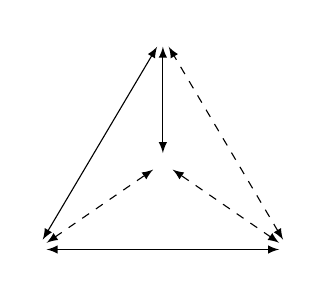
\begin{tikzpicture}
\node (re) at (0,0) {\RE};
\node (dfa) at (0,1.6) {\DFA};
\node (nfa) at (-1.6,-1.1) {\NFA};
\node (enfa) at (1.6,-1.1) {\ENFA};

\draw[latex-latex] (dfa) -- (nfa);
\draw[latex-latex] (nfa) -- (enfa);
\draw[latex-latex, dashed] (enfa) -- (dfa);
\draw[latex-latex] (dfa) -- (re);
\draw[latex-latex, dashed] (nfa) -- (re);
\draw[latex-latex, dashed] (enfa) -- (re);
\end{tikzpicture}
\end{center}
In our diagram, a solid line indicates that we have a method of directly converting between two models of computation, while a dashed line indicates that we have an indirect method---say, by performing two consecutive conversion steps.

All of our conversions considered apart may seem like nothing more than mechanical procedures or unimportant intermediate steps that we can employ in some larger system. However, taken together as we did in our diagram, these conversions reveal what might reasonably be called the most important theorem in the entire study of regular languages.

\begin{theorem}[Kleene's theorem]\label{thm:kleene}
A language $R$ is regular if it satisfies any of the following equivalent properties:
\begin{enumerate}
\item There exists a deterministic finite automaton $\mathcal{M}_{\text{D}}$ such that $L(\mathcal{M}_{\text{D}}) = R$;
\item There exists a nondeterministic finite automaton $\mathcal{M}_{\text{N}}$ such that $L(\mathcal{M}_{\text{N}}) = R$;
\item There exists a nondeterministic finite automaton with epsilon transitions $\mathcal{M}_{\text{E}}$ such that $L(\mathcal{M}_{\text{E}}) = R$; or
\item There exists a regular expression \regex{r} such that $L(\regex{r}) = R$.
\end{enumerate}
\end{theorem}

Note that we don't need to prove anything here---the proof of Kleene's theorem is baked into the descriptions of each of our conversion procedures!
\section{Closure Properties}\label{sec:closurepropertiesregular}

\firstwords{Another important consideration} when we discuss any model of computation is that of \emph{closure properties}, since they allow us to determine whether we can apply certain operations to words or languages while still allowing the same model to accept or recognize the result.

We say that a set $S$ is \emph{closed} under an operation $\circ$ if, given any two elements $a, b \in S$, we have that $a \circ b \in S$ as well. You might be familiar with the notion of closure from elsewhere in mathematics: for example, the set of integers is closed under the operations of addition, subtraction, and multiplication, since for all integers $a$ and $b$, we know that $a + b$, $a - b$, and $a \times b$ are integers. On the other hand, the set of integers is not closed under the operation of division, since (for example) $1, 2 \in \mathbb{Z}$ but $1/2 \not\in \mathbb{Z}$.

We can prove all kinds of closure results for the class of regular languages, but here we will focus only on a few basic operations: the regular operations of union, concatenation, and Kleene star, together with two new set-inspired operations, complement and intersection, which will come in handy later. For each result, we will follow the same general style of proof to establish closure. If the operation $\circ$ is binary, as is the case for union, concatenation, and intersection, then we will take two finite automata $\mathcal{M}$ and $\mathcal{N}$ recognizing languages $L(\mathcal{M})$ and $L(\mathcal{N})$ and directly construct a new finite automaton recognizing the operation language $L(\mathcal{M}) \circ L(\mathcal{N})$. On the other hand, if the operation is unary, as is the case for Kleene star and complement, then we need only take one finite automaton $\mathcal{M}$ recognizing the language $L(\mathcal{M})$ and directly construct a new finite automaton recognizing the operation language $L(\mathcal{M})^{\circ}$.

\subsubsection*{Union}

We begin by considering the union operation. To determine whether some input word belongs to the union of two languages $L(\mathcal{A})$ and $L(\mathcal{B})$, we must check that the word is accepted by either $\mathcal{A}$ or $\mathcal{B}$, or by both. Thus, we must essentially perform two parallel ``subcomputations" for each of these finite automata. This parallelism means we must also incorporate nondeterminism into our computation, since we don't know in advance which of the two finite automata will accept the word.

\begin{theorem}\label{thm:FAclosureunion}
The class of regular languages is closed under the operation of union.

\begin{proof}
Suppose we are given two finite automata, denoted $\mathcal{A} = (Q_{\mathcal{A}}, \Sigma, \allowbreak \delta_{\mathcal{A}}, q_{0_{\mathcal{A}}}, F_{\mathcal{A}})$ and $\mathcal{B} = (Q_{\mathcal{B}}, \Sigma, \delta_{\mathcal{B}}, q_{0_{\mathcal{B}}}, F_{\mathcal{B}})$. We construct a nondeterministic finite automaton with epsilon transitions $\mathcal{C}$ recognizing the language $L(\mathcal{A}) \cup L(\mathcal{B})$ in the following way:
\begin{itemize}
\item Take $Q_{\mathcal{C}} = Q_{\mathcal{A}} \cup Q_{\mathcal{B}} \cup \{q_{0}\}$.
\item Take $q_{0_{\mathcal{C}}} = q_{0}$.
\item Take $F_{\mathcal{C}} = F_{\mathcal{A}} \cup F_{\mathcal{B}}$.
\item Define $\delta_{\mathcal{C}}$ such that, for all $q \in Q_{\mathcal{C}}$ and for all $a \in \Sigma \cup \{\epsilon\}$,
\begin{equation*}
\delta_{\mathcal{C}}(q, a) = 
\begin{cases}
\delta_{\mathcal{A}}(q, a)					& \text{if } q \in Q_{\mathcal{A}}; \\
\delta_{\mathcal{B}}(q, a)					& \text{if } q \in Q_{\mathcal{B}}; \text{ and} \\
\{q_{0_{\mathcal{A}}}, q_{0_{\mathcal{B}}}\}	& \text{if } q = q_{0} \text{ and } a = \epsilon.
\end{cases}
\qedhere
\end{equation*}
\end{itemize}
\end{proof}
\end{theorem}

The ``union" finite automaton $\mathcal{C}$ is depicted in Figure~\ref{subfig:unionautomaton}. Note that, since we now know that all of our models of finite automata are equivalent to one another (and equivalent to regular expressions), the fact that we used nondeterministic finite automata with epsilon transitions in our proof is irrelevant. We did so mainly because it makes the construction easier on us.

\subsubsection*{Concatenation}

Next, we consider the concatenation operation. To determine whether some input word belongs to the concatenation language $L(\mathcal{A})L(\mathcal{B})$, we again need to perform two ``subcomputations" on both finite automata $\mathcal{A}$ and $\mathcal{B}$, but this time in series. The first part of the word should take us to a final state of $\mathcal{A}$, at which point we will jump to $\mathcal{B}$ to read the remaining second part of the word. However, since we don't know where this ``jumping point" is within the word, we again need nondeterminism to guess when we have reached a final state of $\mathcal{A}$.

\begin{theorem}\label{thm:FAclosureconcatenation}
The class of regular languages is closed under the operation of concatenation.

\begin{proof}
Suppose we are given two finite automata, denoted $\mathcal{A} = (Q_{\mathcal{A}}, \Sigma, \allowbreak \delta_{\mathcal{A}}, q_{0_{\mathcal{A}}}, F_{\mathcal{A}})$ and $\mathcal{B} = (Q_{\mathcal{B}}, \Sigma, \delta_{\mathcal{B}}, q_{0_{\mathcal{B}}}, F_{\mathcal{B}})$. We construct a nondeterministic finite automaton with epsilon transitions $\mathcal{C}$ recognizing the language $L(\mathcal{A})L(\mathcal{B})$ in the following way:
\begin{itemize}
\item Take $Q_{\mathcal{C}} = Q_{\mathcal{A}} \cup Q_{\mathcal{B}}$.
\item Take $q_{0_{\mathcal{C}}} = q_{0_{\mathcal{A}}}$.
\item Take $F_{\mathcal{C}} = F_{\mathcal{B}}$.
\item Define $\delta_{\mathcal{C}}$ such that, for all $q \in Q_{\mathcal{C}}$ and for all $a \in \Sigma \cup \{\epsilon\}$,
\begin{equation*}
\delta_{\mathcal{C}}(q, a) = 
\begin{cases}
\delta_{\mathcal{A}}(q, a)							& \text{if } q \in Q_{\mathcal{A}} \text{ and } q \not\in F_{\mathcal{A}}; \\
\delta_{\mathcal{A}}(q, a)							& \text{if } q \in F_{\mathcal{A}} \text{ and } a \neq \epsilon; \\
\delta_{\mathcal{A}}(q, a) \cup \{q_{0_{\mathcal{B}}}\}	& \text{if } q \in F_{\mathcal{A}} \text{ and } a = \epsilon; \text{ and} \\
\delta_{\mathcal{B}}(q, a)							& \text{if } q \in Q_{\mathcal{B}}. \\
\end{cases}
\qedhere
\end{equation*}
\end{itemize}
\end{proof}
\end{theorem}

The ``concatenation" finite automaton $\mathcal{C}$ is depicted in Figure~\ref{subfig:concatenationautomaton}. Again, the fact that we used nondeterministic finite automata with epsilon transitions in this proof does not matter, since any regular language model of computation will work equally well.

\subsubsection*{Kleene Star}

For our next result, pertaining to the Kleene star, we consider just one finite automaton instead of two. However, the construction process is similar to that which we just saw for concatenation. Since the Kleene star is essentially repeated concatenation, upon reaching a final state of the finite automaton $\mathcal{A}$, we will jump backward to allow us to cycle through the computation again if we desire.

There is one technicality, though: we can't jump backward directly to the original initial state of $\mathcal{A}$, since if that initial state has a looping transition, we might be able to mistakenly accept words not in the original language. Thus, we will jump backward to a new state, and from there we can transition to the original initial state of $\mathcal{A}$.

\begin{theorem}\label{thm:FAclosurestar}
The class of regular languages is closed under the operation of Kleene star.

\begin{proof}
Suppose we are given a finite automaton, denoted $\mathcal{A} = (Q_{\mathcal{A}}, \Sigma, \delta_{\mathcal{A}}, \allowbreak q_{0_{\mathcal{A}}}, F_{\mathcal{A}})$. We construct a nondeterministic finite automaton with epsilon transitions $\mathcal{A}'$ recognizing the language $L(\mathcal{A})^{*}$ in the following way:
\begin{itemize}
\item Take $Q_{\mathcal{A}'} = Q_{\mathcal{A}} \cup \{q_{0}\}$.
\item Take $q_{0_{\mathcal{A}'}} = q_{0}$.
\item Take $F_{\mathcal{A}'} = \{q_{0}\}$.
\item Define $\delta_{\mathcal{A}'}$ such that, for all $q \in Q_{\mathcal{A}'}$ and for all $a \in \Sigma \cup \{\epsilon\}$,
\begin{equation*}
\delta_{\mathcal{A}'}(q, a) = 
\begin{cases}
\delta_{\mathcal{A}}(q, a)				& \text{if } q \in Q_{\mathcal{A}} \text{ and } q \not\in F_{\mathcal{A}}; \\
\delta_{\mathcal{A}}(q, a)				& \text{if } q \in F_{\mathcal{A}} \text{ and } a \neq \epsilon; \\
\delta_{\mathcal{A}}(q, a) \cup \{q_{0}\}	& \text{if } q \in F_{\mathcal{A}} \text{ and } a = \epsilon; \text{ and } \\
\{q_{0_{\mathcal{A}}}\}				& \text{if } q = q_{0} \text{ and } a = \epsilon.
\end{cases}
\qedhere
\end{equation*}
\end{itemize}
\end{proof}
\end{theorem}

The ``Kleene star" finite automaton $\mathcal{A}'$ is depicted in Figure~\ref{subfig:kleenestarautomaton} and, again, the usual disclaimer about nondeterministic finite automata with epsilon transitions applies to this proof.

\begin{figure}[p!]
\centering
\begin{subfigure}{\textwidth}
\centering
\begin{tikzpicture}[node distance=2cm, >=latex, every state/.style={fill=white}]
\draw[dashed, draw=\maincolour, fill=\fifthcolour] (1.25,0.3) rectangle (7.25,1.95);
\draw[dashed, draw=\maincolour, fill=\fifthcolour] (1.25,-0.3) rectangle (7.25,-1.95);

\draw[color=\maincolour] (6.9,1.6) node (a) {$\mathcal{A}$};
\draw[color=\maincolour] (6.9,-1.6) node (a) {$\mathcal{B}$};

\node[state, initial] (q0) {$q_{0}$};
\node[state, above right=0.5cm and 1.5cm of q0] (q0a) {$q_{0_{\mathcal{A}}}$};
\node[state, below right=0.5cm and 1.5cm of q0] (q0b) {$q_{0_{\mathcal{B}}}$};
\node[state, right of=q0a, draw=none, fill=none] (qa) {\color{\maincolour}$\dots$};
\node[state, right of=q0b, draw=none, fill=none] (qb) {\color{\maincolour}$\dots$};
\node[state, accepting, right of=qa] (qfa) {};
\node[state, accepting, right of=qb] (qfb) {};

\path[-latex] (q0) edge [bend left, above left] node {$\epsilon$} (q0a);
\path[-latex] (q0) edge [bend right, below left] node {$\epsilon$} (q0b);
\path[-latex] (q0a) edge [above] node {} (qa);
\path[-latex] (q0b) edge [above] node {} (qb);
\path[-latex] (qa) edge [above] node {} (qfa);
\path[-latex] (qb) edge [above] node {} (qfb);
\end{tikzpicture}
\caption{Finite automaton recognizing the union of two languages}
\label{subfig:unionautomaton}
\end{subfigure}

\bigskip
\medskip

\begin{subfigure}{\textwidth}
\centering
\begin{tikzpicture}[node distance=2cm, >=latex, every state/.style={fill=white}]
\draw[dashed, draw=\maincolour, fill=\fifthcolour] (-2,-0.85) rectangle (5.25,0.85);
\draw[dashed, rounded corners, draw=\maincolour, fill=\fourthcolour] (3.35,-0.65) rectangle (4.65,0.65);
\draw[color=\maincolour] (4.95,0.5) node (a) {$\mathcal{A}$};
\draw[color=\thirdcolour] (4.95,-0.5) node (a) {$F_{\mathcal{A}}$};

\node[state, initial] (q0a) {$q_{0_{\mathcal{A}}}$};
\node[state, right of=q0a, draw=none, fill=none] (qa) {\color{\maincolour}$\dots$};
\node[state, right of=qa] (qfa) {};

\path[-latex] (q0a) edge [above] node {} (qa);
\path[-latex] (qa) edge [above] node {} (qfa);

\draw[dashed, draw=\maincolour, fill=\fifthcolour] (1.25,-2.75) rectangle (7.25,-1.05);
\draw[color=\maincolour] (6.9,-2.4) node (b) {$\mathcal{B}$};

\node[state, below=1cm of qa] (q0b) {$q_{0_{\mathcal{B}}}$};
\node[state, right of=q0b, draw=none, fill=none] (qb) {\color{\maincolour}$\dots$};
\node[state, accepting, right of=qb] (qfb) {};

\path[-latex] (q0b) edge [above] node {} (qb);
\path[-latex] (qb) edge [above] node {} (qfb);

\path[-latex] (qfa) edge [above left, pos=0.35] node {$\epsilon$} (q0b);
\end{tikzpicture}
\caption{Finite automaton recognizing the concatenation of two languages}
\label{subfig:concatenationautomaton}
\end{subfigure}

\bigskip

\begin{subfigure}{\textwidth}
\centering
\begin{tikzpicture}[node distance=2cm, >=latex, every state/.style={fill=white}]
\draw[dashed, draw=\maincolour, fill=\fifthcolour] (1.25,-0.85) rectangle (7.25,0.85);
\draw[dashed, rounded corners, draw=\maincolour, fill=\fourthcolour] (5.35,-0.65) rectangle (6.65,0.65);
\draw[color=\maincolour] (6.95,0.5) node (a) {$\mathcal{A}$};
\draw[color=\thirdcolour] (6.95,-0.5) node (a) {$F_{\mathcal{A}}$};

\node[state, initial, accepting] (q0) {$q_{0}$};
\node[state, right of=q0] (q0a) {$q_{0_{\mathcal{A}}}$};
\node[state, right of=q0a, draw=none, fill=none] (qa) {\color{\maincolour}$\dots$};
\node[state, right of=qa] (qfa) {};

\path[-latex] (q0) edge [above, pos=0.35] node {$\epsilon$} (q0a);
\path[-latex] (q0a) edge [above] node {} (qa);
\path[-latex] (qa) edge [above] node {} (qfa);

\path[-latex] (qfa) edge [bend right=40, above] node {$\epsilon$} (q0);
\end{tikzpicture}
\caption{Finite automaton recognizing the Kleene star of a language}
\label{subfig:kleenestarautomaton}
\end{subfigure}
\caption{Finite automaton constructions for each of the three regular operations}
\label{fig:regularoperationautomata}
\end{figure}

\subsubsection*{Complement}

Having established closure for each of the regular operations, we can now shift our focus toward other common language operations, and we will begin by considering the operation of \emph{complement}. Much like with sets, the complement of a language $L$ is a language containing all words that do \emph{not} belong to $L$; that is,
\begin{equation*}
\overline{L} = \{w \mid w \not\in L\}.
\end{equation*}
Thus, to say that regular languages are closed under complement means that, if we were to take a regular language $L$ and consider all words that do \emph{not} belong to $L$, the resultant language would also be regular: perhaps a surprising result at first, but one with a rather easy proof!

\begin{theorem}\label{thm:FAclosurecomplement}
The class of regular languages is closed under the operation of complement.

\begin{proof}
Suppose we are given a deterministic finite automaton $\mathcal{A} = (Q, \Sigma, \delta, q_{0}, F)$. The language of this automaton, $L(\mathcal{A})$, consists of all words that take us from the initial state $q_{0}$ to a final state in the subset $F$. Therefore, the complement of $L(\mathcal{A})$ consists of all words that \emph{do not} take us to a final state.

We construct a finite automaton $\mathcal{A}' = (Q, \Sigma, \delta, q_{0}, F')$ recognizing the language $\overline{L(\mathcal{A})}$ by taking $F' = Q \setminus F$; that is, all non-final states in $\mathcal{A}$ are final states in $\mathcal{A}'$, and vice versa.
\end{proof}
\end{theorem}

Take careful note that, unlike in the previous three closure proofs for union, concatenation, and Kleene star, the closure proof for complement requires that we start with a \emph{deterministic} finite automaton. We cannot simply swap the final and non-final states in a nondeterministic finite automaton and expect the construction to go through with no issues. To see why this is the case, consider the following nondeterministic finite automaton:
\begin{center}
\begin{tikzpicture}[node distance=2cm, >=latex, every state/.style={fill=white}]
\node[state, initial] (q0) {$q_{0}$};
\node[state, accepting, above right of=q0] (q1) {$q_{1}$};
\node[state, below right of=q0] (q2) {$q_{2}$};

\path[-latex] (q0) edge [above left] node {\texttt{a}} (q1);
\path[-latex] (q0) edge [below left] node {\texttt{a}} (q2);
\end{tikzpicture}
\end{center}
Observe that this finite automaton recognizes the singleton language $L = \{\texttt{a}\}$, and so the complement of this finite automaton must \emph{not} include the word \texttt{a} in its language. However, applying our complement construction directly to the nondeterministic finite automaton produces the following result:
\begin{center}
\begin{tikzpicture}[node distance=2cm, >=latex, every state/.style={fill=white}]
\node[state, initial, accepting] (q0) {$q_{0}$};
\node[state, above right of=q0] (q1) {$q_{1}$};
\node[state, accepting, below right of=q0] (q2) {$q_{2}$};

\path[-latex] (q0) edge [above left] node {\texttt{a}} (q1);
\path[-latex] (q0) edge [below left] node {\texttt{a}} (q2);
\end{tikzpicture}
\end{center}
Clearly, this ``complement" finite automaton still accepts the word \texttt{a}! Thus, in order for us to correctly complement a nondeterministic finite automaton, we must first convert it into its equivalent deterministic form.

\subsubsection*{Intersection}

For our last closure result, we will look at the operation of intersection. Recall that, with the union operation, we had to check whether some input word belonged to \emph{either} of the languages $L(\mathcal{A})$ or $L(\mathcal{B})$. With the intersection operation, on the other hand, we must check whether the input word belongs to \emph{both} languages.

We could establish closure via a nice construction known as a \emph{product automaton}, but this isn't strictly necessary. In fact, we can get this new intersection closure result using a couple of the closure results we have already established! This is all thanks to \emph{De Morgan's laws}, one of which allows us to reformulate intersection in terms of both union and complement:
\begin{equation*}
L(\mathcal{A}) \cap L(\mathcal{B}) = \overline{\overline{L(\mathcal{A})} \cup \overline{L(\mathcal{B})}}.
\end{equation*}
Since we already know that the regular languages are closed under union and complement, we get the proof of closure under intersection for free.

\begin{theorem}\label{thm:FAclosureintersection}
The class of regular languages is closed under the operation of intersection.

\begin{proof}
Suppose we are given two deterministic finite automata $\mathcal{A}$ and $\mathcal{B}$ recognizing languages $L(\mathcal{A})$ and $L(\mathcal{B})$, respectively. Since $L(\mathcal{A})$ and $L(\mathcal{B})$ are regular, we know that $\overline{L(\mathcal{A})}$ and $\overline{L(\mathcal{B})}$ are regular by closure under complement. We also know that $\overline{L(\mathcal{A})} \cup \overline{L(\mathcal{B})}$ is regular by closure under union. Therefore, $\overline{\overline{L(\mathcal{A})} \cup \overline{L(\mathcal{B})}}$ is regular again by closure under complement, and so $L(\mathcal{A}) \cap L(\mathcal{B})$ is regular.
\end{proof}
\end{theorem}

\begin{construction}
Eventually, I will detail an alternative approach using the so-called product automaton.
\end{construction}
%\advancedsection{Finite Automata with Output}\label{sec:finiteautomatawithoutput}

\begin{construction}
Eventually, I'll get around to writing this section about finite automata with output. But not today.
\end{construction}

\subsection{Moore and Mealy Machines}

\subsection{Transducers}
\section{Proving a Language is Nonregular}\label{sec:nonregular}

\firstwords{At this point}, it should be evident that finite automata and regular expressions are nice models to use when discussing computation in the abstract. They're easy to define, easy to reason about, and they have a lot of nice properties that we can use in proofs. However, they are not the be-all and end-all of theoretical computer science. (Otherwise, this would be a rather short course!)

Both finite automata and regular expressions suffer the drawback of not having any way to store or recall data. Finite automata don't have any storage mechanism, and regular expressions don't allow for lookback. As we said in the section introducing finite automata, once the finite automaton reads a symbol and transitions to a state, it can never return to that symbol. For all intents and purposes, the symbol is lost forever, and the finite automaton doesn't even remember having read it. Likewise, once a regular expression matches a symbol in a word and moves on to the next symbol, it has no way of remembering any previous symbols that were matched.

Naturally, this means that there exist some languages that cannot be recognized by a finite automaton (or, equivalently, represented by a regular expression), and therefore such languages cannot be regular. For instance, this is the canonical example of a language that no finite automaton can recognize:
\begin{equation*}
L_{\text{a}=\text{b}} = \{\texttt{a}^{n}\texttt{b}^{n} \mid n \geq 0\}.
\end{equation*}
In this language, every word has an equal number of \texttt{a}s and \texttt{b}s, and all occurrences of \texttt{a} appear before the first occurrence of \texttt{b}. Some examples of words in this language are \texttt{ab}, \texttt{aaabbb}, \texttt{aaaaaabbbbbb}, and $\epsilon$.

Why can't any finite automaton recognize this language? Because of that word \emph{finite}. A finite automaton consists of a finite number of states, but in order to recognize this language, we would need to add a ``chain" consisting of $2n + 1$ states to accept the word $\texttt{a}^{n}\texttt{b}^{n}$ for every $n \geq 0$; such a construction is illustrated in Figure~\ref{fig:abequalautomaton}. Since $n$ has no upper bound, we would need an infinite number of states! No finite automaton can recognize this language, because no finite automaton has a way of keeping track of the value $n$ or counting the symbols using only a finite number of states.

\begin{figure}
\centering
\begin{tikzpicture}[node distance=1.75cm, >=latex, every state/.style={fill=white}]
\node[state, initial, accepting] (q0) {$q_{0}$};
\node[state] (q1) [right of=q0] {$q_{1}$};
\node[state, accepting] (q2) [below of=q1] {$q_{2}$};
\node[state, draw=black!80] (q3) [right of=q1] {\color{black!80}$q_{3}$};
\node[state, draw=black!80] (q4) [below of=q3] {\color{black!80}$q_{4}$};
\node[state, draw=black!60] (q5) [right of=q3] {\color{black!60}$q_{5}$};
\node[state, draw=black!60] (q6) [below of=q5] {\color{black!60}$q_{6}$};
\node[state, draw=black!40] (q7) [right of=q5] {\color{black!40}$q_{7}$};
\node[state, draw=black!40] (q8) [below of=q7] {\color{black!40}$q_{8}$};
\node[state, draw=none, fill=none, right of=q7] (qi) {\color{black!20}$\dots$};
\node[state, draw=none, fill=none, right of=q8] (qj) {\color{black!20}$\dots$};

\path[-latex] (q0) edge [above] node {\texttt{a}} (q1);
\path[-latex] (q1) edge [left] node {\texttt{b}} (q2);

\path[-latex] (q1) edge [above] node {\texttt{a}} (q3);
\path[-latex, color=black!80] (q3) edge [left] node {\texttt{b}} (q4);
\path[-latex] (q4) edge [below] node {\texttt{b}} (q2);

\path[-latex, color=black!80] (q3) edge [above] node {\texttt{a}} (q5);
\path[-latex, color=black!60] (q5) edge [left] node {\texttt{b}} (q6);
\path[-latex, color=black!80] (q6) edge [below] node {\texttt{b}} (q4);

\path[-latex, color=black!60] (q5) edge [above] node {\texttt{a}} (q7);
\path[-latex, color=black!40] (q7) edge [left] node {\texttt{b}} (q8);
\path[-latex, color=black!60] (q8) edge [below] node {\texttt{b}} (q6);

\path[-latex, color=black!40] (q7) edge [above] node {\texttt{a}} (qi);
\path[-latex, color=black!40] (qj) edge [below] node {\texttt{b}} (q8);
\end{tikzpicture}
\caption{A ``finite" automaton supposedly recognizing the language $L_{\text{a}=\text{b}}$}
\label{fig:abequalautomaton}
\end{figure}

However, we can't totally rely on the claim that a finite automaton is incapable of recognizing a language if it has to count symbols. For instance, consider the language
\begin{equation*}
L_{\text{a}} = \{\texttt{a}^{n} \mid n \geq 0\}.
\end{equation*}
This language contains an infinite number of words: one word for each $n \geq 0$, exactly like in $L_{\text{a}=\text{b}}$. But it's easy for a finite automaton to recognize $L_{\text{a}}$, and using only one state!
\begin{center}
\begin{tikzpicture}[node distance=2cm, >=latex, every state/.style={fill=white}]
\node[state, initial, accepting] (q0) {$q_{0}$};
\path[-latex] (q0) edge [loop right] node {\texttt{a}} (q0);
\end{tikzpicture}
\end{center}

Thus, it should hopefully be clear that we need to take a slightly more intricate approach in order to prove a language is not regular. There are many more nonregular languages than there are regular languages, so instead of focusing on some sort of property that a nonregular language might have, let's instead find a property every regular language must have. We can then prove a language is nonregular by showing that the language \emph{doesn't} have that property.

\subsection{The Pumping Lemma for Regular Languages}

The property of regular languages that we will make use of is the following: for every regular language, if we take a word in the language of sufficient length, then we can repeat (or \emph{pump}) a middle portion of that word an arbitrary number of times and produce a new word that belongs to the same regular language. This fact is known, appropriately enough, as the \emph{pumping lemma} for regular languages.

\begin{lemma}[Pumping lemma for regular languages]\label{lem:pumpingregular}
For all regular languages $L$, there exists $p \geq 1$ where, for all $w \in L$ with $|w| \geq p$, there exists a decomposition of $w$ into three parts $w = xyz$ such that
\begin{enumerate}
\item $|y| > 0$;
\item $|xy| \leq p$; and
\item for all $i \geq 0$, $xy^{i}z \in L$.
\end{enumerate}
\end{lemma}

Clearly, the pumping lemma contains a lot of notation and terminology to take in at once---not to mention four alternating quantifiers in a row! Let's take a closer look at the lemma from three different perspectives.

\subsubsection*{An Informal Description}

We'll begin by breaking the pumping lemma down piece-by-piece to see what it tells us.
\begin{colouredbox}
\begin{itemize}
\item \textbf{\textit{For all regular languages $\bm{L}$,}} \\ We can take any regular language $L$, and it will satisfy the pumping lemma.
\item \textbf{\textit{there exists $\bm{p \geq 1}$}} \\ Depending on the language $L$, the pumping lemma claims that there exists a constant $p$ for that language. We call $p$ the \emph{pumping constant}.

(If you're curious, $p$ is the number of states in the finite automaton recognizing $L$.)
\item \textbf{\textit{where, for all $\bm{w \in L}$ with $\bm{|w| \geq p}$,}} \\ We can take any word from $L$ with length at least $p$, and it will satisfy the pumping lemma.
\item \textbf{\textit{there exists a decomposition of $\bm{w}$ into three parts $\bm{w = xyz}$}} \\ Depending on the word $w$, the pumping lemma claims that $w$ can be split into three parts, labelled $x$, $y$, and $z$. The $y$ part is what we will use to do the pumping; the $x$ and $z$ parts are just the start and end parts of $w$ that don't get pumped.
\item \textbf{\textit{such that 1.\ $\bm{|y| > 0}$;}} \\ This condition ensures that the $y$ part of $w$ is nonempty, so that we have something to pump.
\item \textbf{\textit{2.\ $\bm{|xy| \leq p}$;}} \\ This condition ensures that there exists some state in the finite automaton recognizing $L$ that is visited more than once, and furthermore, we will visit that state during the computation before we finish reading the part $y$.

(This condition is essentially an application of the pigeonhole principle.)
\item \textbf{\textit{and 3.\ for all $\bm{i \geq 0}$, $\bm{xy^{i}z \in L}$.}} \\ This is the actual pumping part of the pumping lemma. This condition ensures that, no matter how many copies of the $y$ part we include in our word (even zero copies), the resulting word will still belong to the language.
\end{itemize}
\end{colouredbox}

\subsubsection*{A Formal Proof}

Now that we have a greater understanding of what the pumping lemma says, let's take a look at the proof of the lemma. Remember, the property of all regular languages that we're relying on is that if we take a word of sufficient length from the language, then we can pump a middle portion of that word arbitrarily many times and always obtain a word that still belongs to the language. This means that if we consider a finite automaton recognizing that language, there must exist a loop somewhere within that automaton.

\begin{proofbox}[Lemma~\ref{lem:pumpingregular}]
Let $\mathcal{M} = (Q, \Sigma, \delta, q_{0}, F)$ be a deterministic finite automaton recognizing the language $L$, and let $p$ denote the number of states of $\mathcal{M}$.

Take a word $w = w_{1}w_{2} \dots w_{n}$ of length $n$ from $L$, where $n \geq p$, and let $r_{1}, \dots, r_{n+1}$ be the accepting computation of $\mathcal{M}$ on $w$. Specifically, let $r_{i+1} = \delta(r_{i}, w_{i})$ for all $1 \leq i \leq n$. Clearly, this accepting computation has length $n+1 \geq p+1$.

By the pigeonhole principle, there must exist at least two states in the first $p+1$ states of the accepting computation that are the same. Say that the first occurrence of the same state is $r_{j}$ and the second occurrence is $r_{\ell}$. Since $r_{\ell}$ occurs within the first $p+1$ states of the accepting computation, we know that $\ell \leq p+1$.

Decompose the word $w$ into parts $x = w_{1} \dots w_{j-1}$, $y = w_{j} \dots w_{\ell-1}$, and $z = w_{\ell} \dots w_{n}$. As the part $x$ is read, $\mathcal{M}$ transitions from state $r_{1}$ to state $r_{j}$. Likewise, as $y$ is read, $\mathcal{M}$ transitions from $r_{j}$ to $r_{j}$, and as $z$ is read, $\mathcal{M}$ transitions from $r_{j}$ to $r_{n+1}$. Since we are considering an accepting computation, $r_{n+1}$ is a final state, and so $\mathcal{M}$ must accept the word $xy^{i}z$ for all $i \geq 0$. Moreover, we know that $j \neq \ell$, so $|y| > 0$. Lastly, since $\ell \leq p+1$, we have that $|xy| \leq p$. Therefore, all three conditions of the pumping lemma are satisfied.
\end{proofbox}

\begin{figure}[b]
\centering
\begin{tikzpicture}[node distance=2cm, >=latex, every state/.style={fill=white}, decoration={%
      snake,
      segment length=2mm,
      amplitude=0.4mm,
      pre length=4pt,
      post length=4pt,
    }]
\node[state, initial, minimum size=1cm] (q0) {$r_{0}$};
\node[state, minimum size=1cm] (q1) [right of=q0] {$r_{j}$};
\node[state] (qn) [above=0.75cm of q1, draw=none] {$y$};
\node[state, accepting, minimum size=1cm] (q2) [right of=q1] {$r_{n+1}$};

\path[-latex, draw=black, decorate] (q0) -- node[below, yshift=-0.2cm] {$x$} (q1);
\path[-latex, draw=black, decorate] (q1) to[in=50,out=130,looseness=6] (q1);
\path[-latex, draw=black, decorate] (q1) -- node[below, yshift=-0.2cm] {$z$} (q2);
\end{tikzpicture}
\caption{The pumping lemma for regular languages, presented diagrammatically}
\label{fig:pumpinglemma}
\end{figure}

Diagrammatically, this proof can be approximated by Figure~\ref{fig:pumpinglemma}. The wavy transition lines in the figure denote some chain of transitions starting at one state and ending at another state, where we don't care about the states in between. From the figure, we can see that all of the states of the finite automaton between $r_{0}$ and $r_{j}$ are used to read the part $x$, all of the states between $r_{j}$ and $r_{n+1}$ are used to read the part $z$, and there exists a loop of states that both starts and ends with $r_{j}$ that is used to read the part $y$. We can take this loop as many times as we want while reading the input word, and taking one journey around the loop corresponds to ``pumping" the word once.

\subsubsection*{A Fun Game}

Alternatively, we can think of the pumping lemma as an adversarial game, where we're trying to show that some language $L$ is nonregular while our opponent is trying to show that $L$ is, in fact, regular. If we win the game, then $L$ is nonregular, while if our opponent wins, then $L$ is regular. The rules of this game are given in Figure~\ref{fig:pumpinglemmagame}, so that you can play it at the next party you attend.

\begin{figure}
\centering
{\footnotesize
\setlength{\fboxsep}{10pt}
\noindent\fbox{%
\parbox{0.9\textwidth}{%
\vspace{-0.75em}
\begin{center}
\textbf{Rules of the Pumping Lemma Game}
\end{center}
\begin{enumerate}[leftmargin=*]
\item \ul{Your opponent} chooses $p \geq 1$ and claims it is the pumping constant for $L$.
\item \ul{You} choose a word $w \in L$ with $|w| \geq p$ and claim this word can't be decomposed into parts $w = xyz$ that satisfy the three conditions of the pumping lemma.
\item \ul{Your opponent} chooses a decomposition $w = xyz$ such that $|y| \geq 0$ and $|xy| \leq p$, satisfying the first two conditions automatically, and claims that this decomposition will also satisfy the third condition.
\item \ul{You} choose $i \geq 0$ such that $xy^{i}z \not\in L$.
\end{enumerate}
If you complete Step 4, then you win the game!

If you can't find any $i \geq 0$ in Step 4, then you lose the game.

If any of the claims in Steps 1--3 are false, then the person who made the claim loses the game.
}
}
}
\caption{The pumping lemma game}
\label{fig:pumpinglemmagame}
\end{figure}

\subsubsection*{Using the Pumping Lemma}

As we noted, every regular language must satisfy the pumping lemma, and so any language that does not satisfy the pumping lemma must not be regular. This means that we can use the lemma to prove a language is nonregular by contradiction: assuming the language were regular, it should satisfy the pumping lemma, but if we can somehow pump a sufficently long word to produce a word that does \emph{not} belong to the language, our assumption of regularity must not hold.

Even though the pumping lemma looks complex, reducing it to a series of steps as we did here reveals that any proof of the nonregularity of a language simply has to follow each of the steps. As a result, all nonregularity proofs tend to share a similar structure.

Let's take a look at an example of a pumping lemma proof using our canonical nonregular language, $L_{\text{a}=\text{b}}$.

\begin{example}
Let $\Sigma = \{\texttt{a}, \texttt{b}\}$, and consider the language $L_{\text{a}=\text{b}} = \{\texttt{a}^{n}\texttt{b}^{n} \mid n \geq 0\}$. We will use the pumping lemma to show that this language is nonregular.

Assume by way of contradiction that the language is regular, and let $p$ denote the pumping constant given by the pumping lemma. We choose the word $w = \texttt{a}^{p}\texttt{b}^{p}$. Clearly, $w \in L_{\text{a}=\text{b}}$ and $|w| \geq p$. Thus, there exists a decomposition $w = xyz$ satisfying the three conditions of the pumping lemma.

We consider three cases, depending on the contents of the part $y$ of the word $w$:
\begin{enumerate}
\item The part $y$ contains only \texttt{a}s. In this case, pumping $y$ once to obtain the word $xy^{2}z$ results in the word containing more \texttt{a}s than \texttt{b}s, and so $xy^{2}z \not\in L_{\text{a}=\text{b}}$. This violates the third condition of the pumping lemma.

\item The part $y$ contains only \texttt{b}s. In this case, since the first $p$ symbols of $w$ are \texttt{a}s, we must have that $|xy| > p$. This violates the second condition of the pumping lemma.

\item The part $y$ contains both \texttt{a}s and \texttt{b}s. Again, in this case, since the first $p$ symbols of $w$ are \texttt{a}s, we must have that $|xy| > p$. This violates the second condition of the pumping lemma.
\end{enumerate}
In all cases, one of the conditions of the pumping lemma is violated. As a consequence, the language cannot be regular.
\end{example}

Let's step through each component of this proof. We began by assuming our language was regular. From this assumption, the pumping lemma tells us that there exists some value $p \geq 1$ that we can use in our next step: choosing an appropriate word from the language. We choose a word $w$ that is sufficiently long; that is, of length at least $p$. (We chose $\texttt{a}^{p}\texttt{b}^{p}$ here, which makes for a good strategy: try to incorporate the value $p$ into the chosen word in some way.) The pumping lemma then tells us that, since our word $w$ is long enough, there exists some decomposition $w = xyz$ that satisfies the three conditions of the lemma. From here, the remainder of the proof consists of us checking every possible decomposition of $w$ and finding some violated condition for each decomposition.

\begin{dangerous}
Two of the most common mistakes when using the pumping lemma are fixing a specific value for $p$ and choosing a specific decomposition $w = xyz$. We must not do either of these! Fixing a specific value for $p$ is not allowed because the statement of the pumping lemma tells us only that \emph{there exists} a value $p$, not what this value is specifically. Likewise, choosing a specific decomposition is not allowed because the pumping lemma again tells us only that \emph{there exists} a decomposition that satisfies the three conditions. Observe that the example we just saw keeps things as general as possible: it doesn't fix a specific value for $p$, and it considers all possible decompositions before arriving at a conclusion.
\end{dangerous}

A language doesn't necessarily have to count symbols in order to be nonregular. Since finite automata don't have any form of storage, they can't remember symbols they read earlier in an input word. This means that finite automata can't recall parts of a word, and so they can't recognize languages like $L_{\text{double}} = \{ww \mid w \in \Sigma^{*}\}$. Here, we prove that a similar language is nonregular: the language of palindromes, $ww^{\text{R}}$. (The notation $w^{\text{R}}$ denotes the \emph{reversal} of the word $w$.) Palindromes are words that read the same backward as they do forward.

\begin{example}
Let $\Sigma = \{\texttt{a}, \texttt{b}\}$, and consider the language $L_{\text{pal}} = \{ ww^{\text{R}} \mid w \in \Sigma^{*}\}$. We will use the pumping lemma to show that this language is nonregular.

Assume by way of contradiction that the language is regular, and let $p$ denote the pumping constant given by the pumping lemma. We choose the word $w = \texttt{a}^{p}\texttt{bb}\texttt{a}^{p}$. Clearly, $w \in L_{\text{pal}}$ and $|w| \geq p$. Thus, there exists a decomposition $w = xyz$ satisfying the three conditions of the pumping lemma.

Since the second condition of the pumping lemma tells us that $|xy| \leq p$, it must be the case that, in any decomposition, we have $xy = \texttt{a}^{k}$ for some $k \leq p$. Consequently, we have $y = \texttt{a}^{\ell}$ for some $1 \leq \ell \leq k$.

If we pump $y$ once to obtain the word $xy^{2}z$, then we obtain the word $\texttt{a}^{p+\ell}\texttt{bb}\texttt{a}^{p}$, which is no longer a palindrome. This violates the third condition of the pumping lemma. As a consequence, the language cannot be regular.
\end{example}

Lastly, recall the third condition of the pumping lemma: for all $i \geq 0$, $xy^{i}z \in L$. The third condition allows us not only to pump \emph{up} by adding copies of $y$ to the word, but also to pump \emph{down} by removing $y$ from the word. In some cases, pumping down can help us to prove a language is nonregular.

\begin{example}
Let $\Sigma = \{\texttt{a}, \texttt{b}\}$, and consider the language $L_{\text{a}>\text{b}} = \{ \texttt{a}^{i}\texttt{b}^{j} \mid i > j\}$. We will use the pumping lemma to show that this language is nonregular.

Assume by way of contradiction that the language is regular, and let $p$ denote the pumping constant given by the pumping lemma. We choose the word $w = \texttt{a}^{p+1}\texttt{b}^{p}$. Clearly, $w \in L_{\text{a}>\text{b}}$ and $|w| \geq p$. Thus, there exists a decomposition $w = xyz$ satisfying the three conditions of the pumping lemma.

Since the second condition of the pumping lemma tells us that $|xy| \leq p$, it must be the case that, in any decomposition, we have $xy = \texttt{a}^{k}$ for some $k \leq p$. Consequently, we have $y = \texttt{a}^{\ell}$ for some $1 \leq \ell \leq k$.

If we pump $y$ one or more times, then we will always end up with a word that contains more \texttt{a}s than \texttt{b}s, and this word will always belong to the language $L_{\text{a}>\text{b}}$.

However, if we pump $y$ down to obtain the word $xy^{0}z = xz$, then our word will be of the form $\texttt{a}^{p+1-\ell}\texttt{b}^{p}$. Since $\ell \geq 1$, our resultant word has at most as many \texttt{a}s as \texttt{b}s, and so it no longer belongs to the language $L_{\text{a}>\text{b}}$. This violates the third condition of the pumping lemma. As a consequence, the language cannot be regular.
\end{example}

\futuresubsection{The Myhill--Nerode Theorem}

\begin{construction}
Following our discussion of the pumping lemma for regular languages, I will reveal that the pumping lemma doesn't actually work for all languages: there exist nonregular languages that satisfy the lemma's conditions. (See, e.g., \citet*{Ehrenfeucht1981PumpingLemmasRegularSets} and \citet{Johnsonbaugh1990ConversesPumpingLemmas}.) This is because the pumping lemma merely gives a necessary, but not sufficient, condition for regularity. To rectify this, I will talk about the Myhill--Nerode theorem, which gives both necessary and sufficient conditions for regularity.
\end{construction}

\subsubsection*{Summary}

Now that we've established that there exist both regular languages and nonregular languages, we can draw a diagram to represent the theory world as we know it currently. At this point, we're only familiar with two language classes: the class of regular languages and the class of finite languages, which is a subclass of the regular languages that we mentioned very briefly. We also only know about one machine model: finite automata.

\begin{remark}
Finite languages are recognized by a special kind of deterministic finite automaton with no cycles.
\end{remark}

As a result, our diagram in Figure~\ref{fig:chomskyregular} admittedly isn't very interesting right now, but as we continue through future chapters, we will expand and add to it.

\begin{figure}[h]
\centering
\begin{tikzpicture}
\draw[draw=\fourthcolour, fill=\fourthcolour, thick, rounded corners, shift={(2,1)}] (-3,-2) rectangle (3,2);
\draw[draw=\fifthcolour, fill=\fifthcolour, thick, rounded corners, shift={(2,1)}] (-1.75,-1.4) rectangle (1.75,0.6);

\node[color=\maincolour] at (2,1.15) {Finite Languages};
\node[color=\maincolour] at (2,0) {\textit{Acyclic DFAs}};
\node[color=black] at (1,0.6) {$\{\epsilon\}$};
\node[color=black] at (2,0.6) {$\{a\}$};
\node[color=black] at (3,0.6) {$\emptyset$};

\node[color=\maincolour] at (2,2.6) {Regular Languages};
\node[color=\maincolour] at (2,-0.667) {\textit{Finite Automata}};
\node[color=black] at (-0.35,1.25) {$\Sigma^{*}$};
\node[color=black] at (0.25,2) {$\texttt{a} \cup \texttt{ba}$};
\node[color=black] at (2,2) {$\{\texttt{a}, \texttt{b}\}^{*}\texttt{c}$};
\node[color=black] at (3.75,2) {$\texttt{01}^{*} \cup \texttt{1}$};
\node[color=black] at (4.35,1.25) {$\texttt{a}^{n}$};

\node[color=\maincolour] at (0,3.5) {$L_{a>b}$};
\node[color=\maincolour] at (2,3.5) {$\texttt{a}^{n}\texttt{b}^{n}$};
\node[color=\maincolour] at (4,3.5) {$ww^{\text{R}}$};
\end{tikzpicture}
\caption{The hierarchy of language classes and models of computation, as we know it currently}
\label{fig:chomskyregular}
\end{figure}

\unnumberedsection{Chapter Notes}

\firstwords{Many of the references} given here and in later chapters, especially those that pertain to early work in formal languages and automata theory, were sourced from the remarkable and comprehensive survey article written by~\citet{Greibach1981FormalLanguagesOrigins}. For readers who understand French, another in-depth survey article has been published by~\citet{Perrin1995DebutsTheorieAutomates}.

The book chapter by \citet{Yu1997RegularLanguages} provides an excellent starting point for those wanting to learn more about the class of regular languages.

\begin{enumerate}
\item[\ref{sec:regexregularexpressions}.] Regular expressions originated in the work of \citet{Kleene1951RepresentationEvents, Kleene1956RepresentationEvents}, who framed the idea in terms of ``regular events", which are now known as regular languages. Kleene defined three operations on events $E$ and $F$: their ``sum", denoted $E \vee F$; their ``product", denoted $EF$; and the ``iterate of $E$ on $F$", denoted $E^{*}F$. These, in turn, became the regular operations with which we are familiar.

\citet{Brzozowski1962SurveyRegularExpressions} has published a detailed survey on the major results pertaining to regular expressions, many of which we discussed in this chapter.

Although we have used $\epsilon$ here to denote the empty word, some other authors use symbols like $\lambda$ or $\Lambda$ instead. Likewise, you may see the notation $\{\}$ being used to denote the empty language instead of $\emptyset$.

Extended regular expressions, or what we here have called regex, have also been studied in the literature under the name of ``practical regular expressions"; see, for example, the work of~\citet*{Campeanu2003PracticalRegex}. There is a vast body of material on extended regular expressions and their use in the professional world; see, for example, the book by~\citet{Friedl2006MasteringRegularExpressions}. \citet{Cox2007RegexMatchingSimpleFast} discusses how regular expression matching algorithms are implemented and gives a comparative analysis of the performance of such implementations in various programming languages and software tools.

The word ``Kleene" in ``Kleene star" and ``Kleene plus" is pronounced /\textipa{"kleIni}/ (\textsc{klay}-nee), as that's how Stephen Kleene pronounced his last name.\par
\epigraph{As far as I am aware this pronunciation is incorrect\par
in all known languages. I believe that this novel\par
pronunciation was invented by my father.}{Ken Kleene}{as quoted in the entry on ``Stephen Kleene" in the Free On-Line Dictionary of Computing}{}
\vspace{1em}

\item[\ref{sec:finiteautomata}.] The study of finite automata has its origins, of all places, in biology. \citet{McCullochPitts1943LogicalCalculus} were the first to develop a mathematical model of nervous system activity using ideas from propositional logic. Their work on ``nerve nets" laid the foundation for modern research into the applications of neural networks to artificial intelligence.

It seems the first use of the phrase ``theory of automata" came in a symposium talk delivered by \citet{VonNeumann1951GeneralLogicalTheoryAutomata}, where he discussed the direction and future of the then-nascent field. The published version of von~Neumann's talk is interesting since it is followed by a discussion between him and symposium attendees, including McCulloch---one of the authors of the aforementioned ``nerve nets" paper! Von~Neumann spent the final years of his life studying automata theory; for details about his contributions, see the memorial survey written by \citet{Shannon1958VonNeumannAutomataTheory}.

\citet{Kleene1951RepresentationEvents, Kleene1956RepresentationEvents} drew a direct connection between the nerve nets of McCulloch and Pitts and the idea of a finite automaton, and established the fundamental result that a language is ``representable by a nerve net" (i.e., recognized by a finite automaton) if and only if it is a regular language.

\citet{Huffman1954SynthesisSwitchingCircuits, Huffman1954SynthesisSwitchingCircuitsPart2} formalized the notions of states and transition tables (which he called ``flow tables") in the context of analyzing electronic circuits; this work originally appeared in his 1953 doctoral thesis. You may know Huffman better from his work in coding theory and his discovery of \emph{Huffman coding}, which he made as a graduate student.

Building upon Huffman's work, both \citet{Mealy1955MethodSynthesizingCircuits} and \citet{Moore1956GedankenExperiments} investigated further properties of electronic circuits and abstracted the study from circuits to ``representations of circuit requirements", otherwise known as flow charts or finite automata.

Nondeterministic finite automata were introduced by \citet{RabinScott1959FiniteAutomata}, and for this paper Rabin and Scott jointly received the Turing Award in 1976.

As we observed in comparing Figures~\ref{fig:deterministicthirdfromlast} and \ref{fig:deterministicfourthfromlast} to Figures~\ref{fig:nondeterministicthirdfromlast} and \ref{fig:nondeterministicfourthfromlast}, respectively, recognizing the language of words whose $n$th-from-last symbol is \texttt{0} requires $n+1$ states in the nondeterministic case and $2^{n}$ states in the deterministic case. \citet{RabinScott1959FiniteAutomata} first observed an exponential upper bound in the number of states between nondeterministic and deterministic finite automata recognizing the same language, but were uncertain whether this upper bound could be improved. \citet{Moore1971BoundsStateSetSize} showed that the finite automata recognizing these ``$n$th-from-last" languages meet this upper bound exactly. The question of how the size of a finite automaton is affected by converting between models or applying language operations gives rise to the study of \emph{descriptional complexity}, also known as \emph{state complexity}. For more details about this area of research, see the surveys by \citet{HolzerKutrib2011DescriptionalComputationalComplexity} and by \citet*{Gao2016SurveyOperationalStateComplexity}.

Nondeterministic finite automata with epsilon transitions were studied by \citet{OttFeinstein1961DesignSequentialMachines}, although in their paper they referred to such machines as ``improper state diagrams". (For the curious, a ``proper state diagram" to Ott and Feinstein is a deterministic finite automaton.)

\citet{McNaughton1961TheoryOfAutomataSurvey} surveys many of the early major results in automata theory that we have covered here, and also discusses extensions of the model such as probabilistic automata. Readers who would like a more applied introduction to finite automata, with an eye to programming applications and connections to other areas of computer science, may be interested in the survey by \citet{Barnes1972ProgrammersViewAutomata}.

\item[\ref{sec:equivalenceofmodelsregular}.] The idea of using epsilon closure to convert a nondeterministic finite automaton with epsilon transitions into one without was proposed by~\citet{OttFeinstein1961DesignSequentialMachines}.

The subset construction for converting a nondeterministic finite automaton to a deterministic finite automaton is due to~\citet{RabinScott1959FiniteAutomata}. Interestingly, the same fundamental idea was explored independently by~\citet{ChomskyMiller1958FiniteStateLanguages}, one year before the notion of a nondeterministic finite automaton was formalized!

The state elimination algorithm presented here for converting a finite automaton to a regular expression is inspired by that given by~\citet{BrzozowskiMcCluskey1963SignalFlow}.

The McNaughton--Yamada--Thompson algorithm for converting a regular expression to a finite automaton was first published by~\citet{McNaughtonYamada1960RegularExpressionsAutomata} in a purely theoretical context and was later rediscovered by~\citet{Thompson1968RegularExpressionSearch} in the context of compiler theory. In their same paper, McNaughton and Yamada also gave a matrix-based procedure to convert a finite automaton back to a regular expression, but their approach shares the same fundamental idea as the state elimination algorithm.

Kleene's theorem is so named because Kleene established an early equivalence between regular expressions and finite automata in his \citeyear{Kleene1951RepresentationEvents} report. \citet*{Copi1958RealizationEventsLogicalNets} give clearer explications and proofs of Kleene's ``analysis and synthesis theorems" establishing the equivalence. \citet{Lee1960AutomataAndFiniteAutomata} obtained a result matching Kleene's, but using a different abstract machine framework.

\item[\ref{sec:closurepropertiesregular}.] Closure of the class of regular languages under union, concatenation, Kleene star, complement, and intersection was established by~\citet{RabinScott1959FiniteAutomata}. In their paper, Rabin and Scott referred to the concatenation operation as the ``complex product" and the Kleene star operation, perhaps confusingly, as ``closure".

\item[\ref{sec:nonregular}.] The pumping lemma for regular languages was first given by~\citet{RabinScott1959FiniteAutomata}, and also appears in a different form in the paper of~\citet*{BarHillel1961FormalPropertiesPhraseStructureGrammars}.

\citet{Ritchie1963FiniteAutomataSquares} proved that the language of binary squares
\begin{equation*}
L_{\text{sq}2} = \{(n^{2})_{2} \mid (n)_{2} \text{ is the binary representation of } n \in \mathbb{N}\}
\end{equation*}
is not a regular language; as an intermediate step, he shows that the language $\{\texttt{1}^{n}\texttt{0}^{n+1}\texttt{1} \mid n > 0\}$ is nonregular. \citet{Huzino1977ElementaryProofRitchie} give an alternative proof of Ritchie's result.

\citet{Minsky1966UnrecognizableSets} show more generally that any language consisting of a set of binary representations of numbers is nonregular if it violates certain asymptotic density properties; specific examples of nonregular languages they give are
\begin{align*}
L_{k2} &= \{(n^{k})_{2} \mid n \in \mathbb{N} \text{ and } k \geq 1\} \text{ and} \\
L_{\text{primes}2} &= \{(p)_{2} \mid p \text{ is a prime number}\}.
\end{align*}

Although the pumping lemma for regular languages provides only a necessary, but not sufficient, condition for a language to be regular, \citet{Jaffe1978NecessarySufficientPumpingLemma} established a pumping condition for regularity that is both necessary and sufficient.
\end{enumerate}